\documentclass[a4paper, twoside, 12pt]{book}

\usepackage[french]{babel}
%--------------------------
% INPUTENC (encodage du texte)
% FONTENC (positionnement des accents)
%--------------------------
\usepackage[utf8]{inputenc}
%\usepackage{ae,lmodern}
\usepackage[T1]{fontenc}

% Interligne
\usepackage{setspace}

%Pour gérer caractères spéciaux °
\DeclareUnicodeCharacter{00B0}{ }
%Pour les épigraphes
\usepackage{epigraph}
\setlength{\epigraphrule}{0pt}
\setlength{\epigraphwidth}{0.6\textwidth}
 \renewcommand\textflush{flushepinormal}
 \renewenvironment{flushepinormal}{}{\vspace*{-\baselineskip}}

%--------------------------
% HYPERREF (liens hypertextes et métadonnées)
%--------------------------
\usepackage{hyperref}
\hypersetup{%
colorlinks=true,
linkcolor=black,
urlcolor=blue,
citecolor=black
}

\title{Mini-Mémoire}
\author{theophile-miailhe}

%--------------------------
% TOCBIBIND (ajouter la bibliographie dans la Table des matières)
%--------------------------
\usepackage{tocbibind}

%--------------------------
% Éléments de mise en page (marge de 2,5 cm, alinéa en début de paragraphe 1cm, interligne 1,5)
%--------------------------
\usepackage[a4paper, margin=2.5cm]{geometry}
\usepackage{setspace}
\onehalfspacing
\setlength{\parindent}{1cm}

\usepackage{fancyhdr}
\setlength{\headheight}{28pt}
\renewcommand{\chaptermark}[1]{\markboth{#1}{}}
\renewcommand{\sectionmark}[1]{\markright{#1}}
\pagestyle{fancy}
\fancyhf{}
\fancyhead[LE,RO]{\thepage}
\fancyhead[LO]{\nouppercase{\rightmark}}
\fancyhead[RE]{\nouppercase{\leftmark}}
\renewcommand{\headrulewidth}{0pt}

%--------------------------
% Modules pour gérer les listes
%--------------------------
\usepackage{enumerate}
\usepackage{enumitem}


%--------------------------
% BIBLIOGRAPHIE
%--------------------------
\usepackage[backend=biber, sorting=nyt, style=enc]{biblatex}
\usepackage[autostyle]{csquotes}

%\bibliography{mybibliography.bib}
\addbibresource{biblio_temp_tech.bib}


\setcounter{secnumdepth}{5}
\setcounter{tocdepth}{2}

\usepackage[official]{eurosym}
\usepackage{afterpage}

%--------------------------
% FIGURES
%--------------------------
\usepackage{graphicx}
\graphicspath{ {./Images} }
\usepackage{float}
\usepackage{longtable}
\usepackage{csvsimple}
\usepackage{changepage}

% ============================================

\begin{document}

\frontmatter
\begin{titlepage}
\begin{center}

\bigskip

\begin{large}
UNIVERSITÉ PARIS, SCIENCES \& LETTRES
\end{large}

\begin{center}\rule{2cm}{0.02cm}\end{center}

\bigskip
\bigskip
\bigskip
\begin{Large}
\textbf{Theophile Miailhe}\\
\end{Large}
\begin{normalsize}
\end{normalsize}

\bigskip
\bigskip
\bigskip

\begin{Huge}
\textbf{Les soldats d'un conflit oublié}\\
\end{Huge}

\bigskip
\bigskip
\begin{LARGE}
\textbf{Une étude statistique des morts de la Guerre du Rif: 1925 - 1926}\\
\end{LARGE}

\bigskip
\bigskip
\bigskip
\vfill

\begin{large}
Mémoire de première année du master\\
\og Humanités Numériques \fg{} \\
\bigskip
2022
\end{large}

\end{center}
\end{titlepage}

\section*{Résumé}
\addcontentsline{toc}{chapter}{Résumé}
 Il existe un manque important dans l'historiographie du Maroc et de l'empire français au sujet du sort des troupes coloniales et metropolitaines pendant la guerre du Rif. L'objectif de ce rapport est de mettre en lumière l'histoire et la trajectoire des differents régiments qui ont participé à cette guerre. Les méthodes quantitatives nous permettent de réaliser une étude statistique ainsi qu'une géographie économique des ces soldats. Nous utilisons des méthodes classiques de sciences des données afin de completer les sources qualitatives dont nous disposons sur cette guerre. 

\medskip

\textbf{Mots-clés: méthodes quantitatives ; géographie économique ; base de données ; armée de terre ; histoire militaire ; histoire coloniale ; humanités numériques ; HTR}

\textbf{Informations bibliographiques:} Theophile Miailhe, \textit{Les soldats d'un conflit oublié : Une étude statistique des morts de la Guerre du Rif: 1925 - 1926}, mémoire de master 1 \og Humanités Numériques\fg{}, dir. [Nicolas Mariot, Julian Randon-Furling], Université Paris, Sciences \& Lettres, 2022.


\section*{Abstract}
\addcontentsline{toc}{chapter}{Abstract}
The historiography of Morocco and France's colonial empire is rather shallow on the subject of the the French army's involvement in the Rif War. The objective of this dissertation is to highlight the diversity of regiments  that participated in the Rif War and the maintenance of France's colonial empire. Quantitative methods allow us to dissect and group soldiers in more precise ways, which would have been time consuming and costly in the past. The marriage of both quantitative and qualitative sources aims to provide new insights on the conflict. 

\medskip

\textbf{Keywords: quantitative history ; databases ; military history ; colonial history ; digital humanities ; HTR}

\textbf{Bibliographic Information:} Theophile Miailhe, \textit{Soldiers of a forgotten war: a quantative approach to the Rif campaign: 1925 - 1926}, M.A. thesis \og Digital Humanities\fg{}, dir. [Nicolas Mariot, Julian Randon-Furling], Université Paris, Sciences \& Lettres, 2022.

\clearpage

\mainmatter

\part*{Introduction}
\addcontentsline{toc}{part}{Introduction}
\markboth{Introduction}{Introduction}
Force est de constater que le débat sur la mémoire des guerres mondiales et la colonisation est plus que jamais d’actualité sur la scène politique française. Si les historiens ont travaillé sur la question de la contribution de l'empire français aux deux guerres mondiales, des conflits de moindre ampleur sont restés largement oubliés. Les réponses à ces questions ne sont pas si évidentes, surtout si l'on tient compte des différentes guerres de l’histoire contemporaine française dans lesquelles les  troupes coloniales ont été engagées depuis la période napoléonienne. Il n'y a pas de consensus sur  la question des soldats morts pendant la guerre du Rif. L’historiographie tend vers une réponse qui place les pertes des soldats nord-africains et de la coloniale au-dessus de celles des soldats métropolitains.\footcites{schiavon2016} Mais cette thèse n’est pas hégémonique car la guerre a connu différentes phases avec des moyens et des concentrations de troupes très variés, et la participation des différentes composantes n'a jamais été quantifiée. L’histoire de cette guerre a souvent été oubliée mais elle suscite aujourd'hui un regain d'intérêt , probablement en raison de son caractère unique et prémonitoire.\footcites{marly2021} La guerre du Rif a été un précurseur des guerres post-coloniales car c'est  la première guerre du 20eme siècle où un peuple indigène a cherché  à se débarrasser de son colonisateur européen. C'est aussi  la première guerre moderne dans le sens où elle a intégré  l’aviation, les chars et l'utilisation d'armes  chimiques (de manière systématique  par l’armée espagnole). Elle peut donc  être considérée comme la première « opération extérieure »\footnote{Le terme contemporain désignant le déploiement de soldats français hors de la metropole.} de l’armée française. En fait, sa caractérisation fluctue entre celle d’une guerre de conquête coloniale, d’une guerre de décolonisation et d’une guerre post-coloniale. Si la guerre du Rif est riche d'enseignements sur l'histoire de l'armée française et son rapport au colonialisme, elle est également révélatrice des fondements de la société marocaine qui perdurent encore aujourd'hui.\\  

Les montagnes du Rif au Maroc ont une longue histoire de contestation sociale, qui remonte à avant l'arrivée du pouvoir français dans le pays. La guerre du Rif de 1921 à 1926 fait partie de l’histoire mouvementée de cette région. Le bilan anthropologique du Rif réalisé par Khalid Mouna expose la singularité du cas Rifain dans le paysage Marocain. Cependant une comparaison approfondie avec des études sociologiques d’autres régions berbères du Maghreb ne permet pas de distinguer spécifiquement ce cas. C’est en effet la situation agricole dans le Rif qui a façonné les relations entre ses habitants et son histoire.\footcites[101]{mouna2008} Historiquement surpeuplé et ayant des terres pauvres, différents sociologues, de Bourdieu à Jamous, se sont penchés sur la prétendue anarchie qui régit le Rif. Les mouvements sociaux  dans le Rif peuvent et doivent être placés dans un contexte régional. Le soulèvement de 1958 et le mouvement populaire du Rif en 2016-2017 montrent que les tensions entre le pouvoir central marocain et les habitants du Rif n’ont pas disparu avec la fin du protectorat. L'œuvre d’Ibn Khaldun, \underline{La Muqaddima}, affirme l’idée que la perspective historique est fondamentale afin de comprendre les changements que peut connaître une société.\footcites[103]{mouna2008}  Quand Mouna essaye d’appliquer ce qu’il qualifie d’une « démarche khaldounienne » à ces questions, nous pouvons constater la continuité du même rôle que le Rif joue à travers l’histoire. C’est dans cette veine  que Mouna explique les liens puissants entre le Rif et la production du kif (résine de cannabis).\footcites[105]{mouna2008} Un saint-homme, fondateur de la confrérie soufie Haddawa, Sidi Haddi s’est installé dans la tribu des Ketama dans le Rif central, au début 19eme siècle. Cette confrérie est la seule à prôner l'usage du cannabis dans un cadre islamique. Quand on sait que la quasi-totalité de la culture du cannabis au Maroc aujourd’hui se situe dans le Rif, les liens entre la guerre du Rif et la culture de contrebande et des hors-la-loi peuvent paraître plus clairs.\footcites{chouvy2007} D’autant plus que des historiens espagnols ont démontré à quel point le Rif et l'Espagne ont été complices dans le trafic d'armes et de contrebande tout au long de la guerre.\\


La guerre du Rif a commencé en 1921, quand les Espagnols ont été vaincus à la bataille d’Anoual par l’armée rifaine d’Abdelkrim. Le conflit a éclaté à la suite d’une nouvelle politique sur  le territoire de leurs comptoirs marocains : les militaires espagnols ayant décidé de quitter la plaine pour installer des postes dans le massif du Rif, territoire des rifains, un peuple farouchement indépendant et belliqueux.\footcites[32]{ayache1996} Après un début catastrophique pour l’armée espagnole, la situation se stabilise  jusqu'en 1925, lorsque les Rifains attaquent le territoire français dans la partie sud des montagnes du Rif. C’est lorsque Abdelkrim lance son offensive vers le nord du protectorat français, que la guerre du Rif commence réellement. Elle va durer de 1925 à 1926 pour les Français jusqu’à la reddition d' Abdelkrim en mai 1926. Il est utile pour pouvoir analyser  les archives de comprendre que durant  cette période, la guerre a connu trois phases  différentes : ce que les militaires appellent la période « héroïque » (avril à août 1925), la période de stabilisation du front (septembre 1925 à avril 1926), et la période de guerre totale (mars à mai 1926).\footcites[79]{schiavon2016} Le début de la guerre est appelé la période « héroïque » car l’armée française a subi ses plus grandes pertes pendant cette phase de la guerre. Elle est en sous-effectif et elle doit  manoeuvrer et combattre sur tout le territoire du protectorat pour contenir les débordements rifains. La période de stabilisation du front porte ce nom parce qu’il décrit ce qui s’est passé pendant que les Français préparaient une offensive majeure. La période de guerre totale correspond à l'arrivée du maréchal Pétain au pouvoir en France et à une augmentation considérable des troupes et des moyens matériels de l’armée française au Maroc. L’armée française subit très peu de pertes pendant cette offensive. Connaître ces trois périodes est utile car elles sont censées correspondre aux éléments chiffrées des pertes dans les bases de données des archives. \\


La littérature secondaire sur la guerre du Rif est étonnamment mince. La tendance la plus répandue dans  l’historiographie se concentre sur les effets de la guerre sur la politique espagnole. Cette tendance est prédominante en raison  de la position centrale que la guerre a joué dans l'ascension de Franco et la future guerre civile espagnole. Les historiographies anglaise et espagnole sont dominées par ce point de vue.\footcites{harris1925} En revanche, les historiographies  française et marocaine accordent plus d'importance  à l’étude du phénomène Rifain et à la République d’Abdelkrim. La littérature secondaire française se concentre sur le rôle de l’armée, des politiques et des grandes figures qui ont mené  la guerre (Lyautey et Pétain). Elle s'intéresse très sporadiquement à inscrire la guerre dans une logique coloniale en étudiant les différentes composantes de l’empire qui y ont participé. \\


Sur le plan numérique et quantitatif, il n’existe à ma connaissance qu’un seul article qui traite de la guerre du Rif en humanités numériques : le travail d’analyse des réseaux de Julián López sur la contrebande pendant la guerre du Rif.\footcites{lopez2016} En histoire militaire dans la période 14-18, Henri Gilles, Jean-Pascal Guironnet, et Antoine Parent ont réalisé une étude proche  de celle que j’envisage de faire sur la \underline{« Géographie économique des morts de 14-18 en France »}.  À partir d'une base de données du SHD de la Première guerre mondiale, ils ont essayé de dénombrer et de trier les individus Morts pour la France (MPF) par régions et de comparer les données MPF avec celles du recensement de 1911. Cela leur a permis d'extrapoler un calcul des décès en proportion des mobilisables par région.\footcites[521]{gilles2014} Ils ont ensuite construit un modèle pour expliquer  la différence en proportions de pertes de chaque région. Pour représenter cet indicateur, ils ont imaginé les deux effets qui pouvaient y contribuer : le taux de mobilisables et la densité de population. En multipliant ces deux facteurs, ils sont arrivés avec l’indicateur des mobilisables par surface :
$
\frac{mobilisables}{surface} = 
\frac{mobilisables}{population}* 
\frac{population}{surface}. 
$\footcites[523]{gilles2014}
Ils ont aussi essayé de créer un modèle dit « historique » qui prend en compte les variables géographiques (distance au front ou à la frontière) ou le taux de ruralité dans la région.\\


En contrepartie,dans \underline{Tous égaux devant « l’impôt du sang» ?} de la même revue, André Loez et Nicolas Mariot, replacent l’article précédent dans son contexte historiographique (par rapport à l’histoire quantitative et celle de 14-18) et contestent l’utilisation anachronique des régions choisies pour des données qui n’étaient pas dans ce format originel. L’autre problème souligné par Mariot et Loez est la question des âges auxquels les hommes étaient mobilisables. L’article de Gilles, Guironnet et Parent utilise les âges légaux de mobilisation mais il y a une proportion importante d’hommes qui n'étaient pas dans cette tranche d'âges mais qui ont quand même combattu, ce qui fausse leur proportion de morts par mobilisables.\footcites[538]{mariot2014} Bien que les deux auteurs apprécient la tentative de modélisation , ils concluent sans ambages à son caractère endémique dans l'historiographie de la Première Guerre mondiale. Elle  manque de données brutes, d’informations sur la manière dont ils sont parvenus à  ses résultats et de réponses aux questions de l'historiographie de la Première Guerre mondiale.\footcites[541]{mariot2014}\\


La dichotomie entre ces deux publications a révélé l'indissociabilité de la méthodologie et de la problématique, et va ainsi me servir de guide pour ma propre étude.  Ma problématique est de faire la lumière sur les différents régiments coloniaux et métropolitains qui ont été amenés à servir pendant la guerre du Rif et de situer les résultats de mon étude dans l’historiographie manquante de ce conflit. 







\part{Présentation des sources primaires}
\chapter{}
\section{Presentation}
Pour répondre à cette problématique, j’ai à ma disposition trois types de sources primaires:
\begin{itemize}
 \item{Les données de la base des « Militaires décédés sur les théâtres d'opérations extérieurs (1905-1962) ».\footnote{\url{https://www.memoiredeshommes.sga.defense.gouv.fr/fr/article.php?larub=46&titre=militaires-decedes-sur-les-theatres-d-operations-exterieurs-1905-1962-}}}
\item{Les registres matricules, qui sont numérisés sur le site \underline{Mémoire des hommes} mais seulement jusqu'à 1918.\footnote{\url{https://www.memoiredeshommes.sga.defense.gouv.fr/fr/article.php?larub=382&titre=recensement-des-engages-et-appeles-des-anciennes-colonies-francaises}}}
\item{Les journaux des marches et opérations des régiments ayant participé à la guerre du Rif, qui ne sont pas numérisés.\footnote{Dans les fonds du SHD sur la Maroc (serie 3H).}}
\end{itemize}
Il existe sûrement d’autres documents d’archives qui traitent de la pluralité des soldats ayant participé à la guerre du Rif dans les archives des officiers supérieurs, généraux, administrateurs et personnalités qui ont contribué à la conduite de la guerre et à l’administration du protectorat du Maroc. Au niveau individuel et à grande échelle, je ne dispose que ses trois objets historiques.\\ 
\section{La base de données de morts}
Cette base de données devrait contenir tous les morts de l’armée française en dehors du sol national pendant la période spécifiée (1905-1962). Ces dates correspondent au début des affrontements entre le Maroc et la France et à la fin de la guerre de l’Algérie. Après cette période, lors de la création de la Vème République, le concept d'opération extérieure a été  créé pour désigner les conflits et opérations des armées françaises en dehors de la métropole. Avant la création du concept, les forces armées françaises ont entrepris des opérations très  variées sans nom particulier . Elles pouvaient se dérouler  en territoire ennemi comme l’Allemagne, ou encore en Russie pendant la guerre civile ou au Maroc ou alors sur un autre territoire de l’empire français. Ce que j’essaie de souligner, est que la terminologie «opérations extérieures » de cette base de données ne correspond à aucune nomenclature militaire ou politique. Ce manque d'homogénéité dans la nature  des opérations menées incluses dans cette base est visible dans sa composition diplomatique. Les informations contenues dans la base proviennent de plusieurs types de documents tels que des fiches individuelles de décès ou des statuts de pension militaire. Pour être encore plus précis, elles proviennent de deux archives spécifiques du SHD : la Division des Archives des Victimes des Conflits Contemporains (DAVCC) du Service historique de la défense à Caen et les archives de la sous-direction des pensions militaires à la Rochelle. À partir de la réunion des fonds des côtes 40 R, 35 R et 36 R pour les fiches individuelles de décès en provenance de la DAVCC et de fonds inconnus des pensions militaires de la Rochelle, une équipe sous la direction de Christophe Dupont a procédé à la transcription et l’encodage de la base de données en question qui a été publiée en 2012. Depuis sa mise en ligne, la base a continué à évoluer avec des mises à jour périodiques de nouvelles données. Grâce à un travail de volontariat des internautes, les informations manquantes ont pu être complétées avec des fiches de matricules. Du coup la base n’est plus évolutive aujourd’hui. \footnote{Information provenant d’un entretien téléphonique avec la  Division des Archives des Victimes des Conflits Contemporains du SHD, de Caen, un échange par mail avec M. Christophe Dupont (24/05/2022) et du site \href{https://www.memoiredeshommes.sga.defense.gouv.fr/fr/article.php?laref=69&titre=aide-a-la-recherche}{\underline{Mémoire des hommes}}. }\\

Comme pour l'ensemble du site Mémoire des hommes, le SHD utilise le logiciel de gestion de site web et données d’archives publiques proposé par l’entreprise \href{http://www.arkotheque.fr/}{\underline{Arkothèque}}. Cette interface permet de télécharger et de naviguer dans la base de données selon plusieurs critères : ceux de l’état civil du soldat décédé, et si le cas le permet, des détails plus précis comme le conflit où il a combattu,et les détails de sa mort ou son grade. Elle permet aussi de différencier les titres que la hiérarchie militaire a attribués à la mort de chacun des ces soldats, par exemple: « mort pour la France », non-statué ou inconnu. Ces recherches sont effectuées avec le moteur d’Arkothèque qui fonctionne sur la  base de \textbf{javascript}.\footnote{Voir annexe : \ref{fig:Arkothèque 1}, \ref{fig:Arkothèque 2}.} Cela limite les possibilités de faire un scrapping ciblé de la base de données. Heureusement, la base de données peut être téléchargée sous format CSV. La figure 1 représente un échantillon réduit du tableau brut de la base de données.\begin{figure}[H]
    \hspace*{-2cm} 
    \caption{La base de données en format CSV}
    \label{fig:1}
     \begin{adjustwidth}{-2cm}{}
\begin{longtable}[c]{llllllllllllllllllllllllllllllllllllllllllllllllllllllllllllllllllllllllll}
id\_conflit\_intitule & id\_sous\_conflit\_intitule & id\_famille\_cote\_intitule & sous\_serie & serie & article & nom & prenom & nom\_autre & pseudonyme & naissance\_jour\_mois\_annee & id\_naissance\_lieu\_intitule & id\_naissance\_departement\_intitule & id\_naissance\_pays\_intitule & id\_statut\_intitule & id\_mention\_intitule & classe & recrutement\_matricule & id\_recrutement\_bureau\_intitule & id\_grade\_intitule & id\_unite\_intitule & id\_bataillon\_intitule & id\_compagnie\_intitule & id\_batterie\_intitule & detail\_unite & id\_profession\_intitule & deces\_jour\_mois\_annee & id\_deces\_lieu\_intitule & id\_deces\_departement\_intitule & id\_deces\_pays\_intitule & id\_operation\_intitule & id\_transcription\_etablissement\_lieu\_intitule & id\_transcription\_etablissement\_departement\_intitule & id\_transcription\_etablissement\_pays\_intitule & id\_dernier\_domicile\_lieu\_intitule & id\_dernier\_domicile\_departement\_intitule & id\_dernier\_domicile\_pays\_intitule & id\_sepulture\_lieu\_intitule & id\_sepulture\_departement\_intitule & id\_sepulture\_pays\_intitule & id\_sepulture\_nom\_du\_site\_intitule & id\_sepulture\_type\_intitule & sepulture\_carre & sepulture\_rang & sepulture\_tombe\_individuelle\_numero & sepulture\_tombe\_indice & id\_sepulture\_lieu\_premiere\_inhumation\_intitule & id\_lieu\_incarceration\_intitule & sources & cote & id\_region\_militaire\_intitule & deportation & id\_decoration\_intitule & decoration\_posthume & decret & jo & id\_mdh\_base\_nominative\_lien\_famille\_resistance\_les\_intitules & id\_mdh\_base\_nominative\_lien\_nom\_mouvement\_rif\_les\_intitules & id\_mdh\_base\_nominative\_lien\_nom\_reseau\_ffc\_les\_intitules & rehabilitation & rehabilitation\_detail & site\_conservation & lien\_ark\_fiche & corps\_retrouve & disparition\_date\_libre & disparition\_jour\_mois\_annee & jdd\_jour\_mois\_annee & disparition\_lieu\_complement & id\_disparition\_lieu\_intitule & id\_disparition\_departement\_intitule & id\_disparition\_pays\_intitule & id\_tgi\_lieu\_intitule & id\_tgi\_departement\_intitule & id\_tgi\_pays\_intitule \\
\endfirsthead
%
\endhead
%
Théâtres d'opérations extérieurs & Afrique du Nord &  &  &  &  & AB EL OUAHAB BEN SAID BEN BELGACEM &  &  &  & 0000-00-00 &  &  &  &  & Non Mort pour la France &  &  &  & soldat & 20e régiment de tirailleurs (20e RT) &  &  &  &  &  & 08/10/1925 & Taza &  & Maroc &  &  &  &  &  &  &  &  &  &  &  &  &  &  &  &  &  &  & Service historique de la Défense, Caen &  &  & 0 &  & 0 &  &  &  &  &  & 0 &  &  & https://www.memoiredeshommes.sga.defense.gouv.fr/fr/ark:/40699/m00523bec44c8132 & 0 &  &  &  &  &  &  &  &  &  &  \\
Théâtres d'opérations extérieurs & Levant & AC & 40 & R & 4063 & ABABOA &  &  &  &  &  &  &  &  & Non Mort pour la France &  &  &  & soldat &  &  &  &  &  &  & 19/07/1920 & Tarsous &  & Cilicie &  & Lavigerie &  & Algérie &  &  &  &  &  &  &  &  &  &  &  &  &  &  & Service historique de la Défense, Caen &  &  & 0 &  & 0 &  &  &  &  &  & 0 &  &  & https://www.memoiredeshommes.sga.defense.gouv.fr/fr/ark:/40699/m00523be53d49952 & 0 &  &  &  &  &  &  &  &  &  &  \\
Théâtres d'opérations extérieurs & Levant & AC & 40 & R & 4063 & ABABOU & Abdelkader &  &  &  &  &  &  &  & Non Mort pour la France &  &  &  & sergent & 18e régiment de tirailleurs (18e RT) &  &  &  &  &  & 11/04/1920 & Ourfa &  & Cilicie &  & Les Attafs &  & Algérie &  &  &  &  &  &  &  &  &  &  &  &  &  &  & Service historique de la Défense, Caen &  &  & 0 &  & 0 &  &  &  &  &  & 0 &  &  & https://www.memoiredeshommes.sga.defense.gouv.fr/fr/ark:/40699/m00523be2909f48a & 0 &  &  &  &  &  &  &  &  &  &  \\
Théâtres d'opérations extérieurs & Afrique du Nord & AC & 40 & R & 4034 & ABABSA & Belgacem &  &  &  &  &  &  &  & Non Mort pour la France &  &  &  & soldat & 11e régiment de tirailleurs (11e RT) &  &  &  &  &  & 16/08/1923 & Ahl Telt &  & Maroc &  & Khenchela (ex département de Constantine) &  & Algérie &  &  &  &  &  &  &  &  &  &  &  &  &  &  & Service historique de la Défense, Caen &  &  & 0 &  & 0 &  &  &  &  &  & 0 &  &  & https://www.memoiredeshommes.sga.defense.gouv.fr/fr/ark:/40699/m00523be18c4cba3 & 0 &  &  &  &  &  &  &  &  &  & 
\end{longtable}
\begin{longtable}[c]{llllllllllllllllllllllllllllllllllllllllllllllllllllllllllllllllllllll}
serie & article & nom & prenom & nom\_autre & pseudonyme & naissance\_jour\_mois\_annee & id\_naissance\_lieu\_intitule & id\_naissance\_departement\_intitule & id\_naissance\_pays\_intitule & id\_statut\_intitule & id\_mention\_intitule & classe & recrutement\_matricule & id\_recrutement\_bureau\_intitule & id\_grade\_intitule & id\_unite\_intitule & id\_bataillon\_intitule & id\_compagnie\_intitule & id\_batterie\_intitule & detail\_unite & id\_profession\_intitule & deces\_jour\_mois\_annee & id\_deces\_lieu\_intitule & id\_deces\_departement\_intitule & id\_deces\_pays\_intitule & id\_operation\_intitule & id\_transcription\_etablissement\_lieu\_intitule & id\_transcription\_etablissement\_departement\_intitule & id\_transcription\_etablissement\_pays\_intitule & id\_dernier\_domicile\_lieu\_intitule & id\_dernier\_domicile\_departement\_intitule & id\_dernier\_domicile\_pays\_intitule & id\_sepulture\_lieu\_intitule & id\_sepulture\_departement\_intitule & id\_sepulture\_pays\_intitule & id\_sepulture\_nom\_du\_site\_intitule & id\_sepulture\_type\_intitule & sepulture\_carre & sepulture\_rang & sepulture\_tombe\_individuelle\_numero & sepulture\_tombe\_indice & id\_sepulture\_lieu\_premiere\_inhumation\_intitule & id\_lieu\_incarceration\_intitule & sources & cote & id\_region\_militaire\_intitule & deportation & id\_decoration\_intitule & decoration\_posthume & decret & jo & id\_mdh\_base\_nominative\_lien\_famille\_resistance\_les\_intitules & id\_mdh\_base\_nominative\_lien\_nom\_mouvement\_rif\_les\_intitules & id\_mdh\_base\_nominative\_lien\_nom\_reseau\_ffc\_les\_intitules & rehabilitation & rehabilitation\_detail & site\_conservation & lien\_ark\_fiche & corps\_retrouve & disparition\_date\_libre & disparition\_jour\_mois\_annee & jdd\_jour\_mois\_annee & disparition\_lieu\_complement & id\_disparition\_lieu\_intitule & id\_disparition\_departement\_intitule & id\_disparition\_pays\_intitule & id\_tgi\_lieu\_intitule & id\_tgi\_departement\_intitule & id\_tgi\_pays\_intitule \\
\endfirsthead
%
\endhead
%
 &  & AB EL OUAHAB BEN SAID BEN BELGACEM &  &  &  & 0000-00-00 &  &  &  &  & Non Mort pour la France &  &  &  & soldat & 20e régiment de tirailleurs (20e RT) &  &  &  &  &  & 08/10/1925 & Taza &  & Maroc &  &  &  &  &  &  &  &  &  &  &  &  &  &  &  &  &  &  & Service historique de la Défense, Caen &  &  & 0 &  & 0 &  &  &  &  &  & 0 &  &  & https://www.memoiredeshommes.sga.defense.gouv.fr/fr/ark:/40699/m00523bec44c8132 & 0 &  &  &  &  &  &  &  &  &  &  \\
R & 4063 & ABABOA &  &  &  &  &  &  &  &  & Non Mort pour la France &  &  &  & soldat &  &  &  &  &  &  & 19/07/1920 & Tarsous &  & Cilicie &  & Lavigerie &  & Algérie &  &  &  &  &  &  &  &  &  &  &  &  &  &  & Service historique de la Défense, Caen &  &  & 0 &  & 0 &  &  &  &  &  & 0 &  &  & https://www.memoiredeshommes.sga.defense.gouv.fr/fr/ark:/40699/m00523be53d49952 & 0 &  &  &  &  &  &  &  &  &  &  \\
R & 4063 & ABABOU & Abdelkader &  &  &  &  &  &  &  & Non Mort pour la France &  &  &  & sergent & 18e régiment de tirailleurs (18e RT) &  &  &  &  &  & 11/04/1920 & Ourfa &  & Cilicie &  & Les Attafs &  & Algérie &  &  &  &  &  &  &  &  &  &  &  &  &  &  & Service historique de la Défense, Caen &  &  & 0 &  & 0 &  &  &  &  &  & 0 &  &  & https://www.memoiredeshommes.sga.defense.gouv.fr/fr/ark:/40699/m00523be2909f48a & 0 &  &  &  &  &  &  &  &  &  &  \\
R & 4034 & ABABSA & Belgacem &  &  &  &  &  &  &  & Non Mort pour la France &  &  &  & soldat & 11e régiment de tirailleurs (11e RT) &  &  &  &  &  & 16/08/1923 & Ahl Telt &  & Maroc &  & Khenchela (ex département de Constantine) &  & Algérie &  &  &  &  &  &  &  &  &  &  &  &  &  &  & Service historique de la Défense, Caen &  &  & 0 &  & 0 &  &  &  &  &  & 0 &  &  & https://www.memoiredeshommes.sga.defense.gouv.fr/fr/ark:/40699/m00523be18c4cba3 & 0 &  &  &  &  &  &  &  &  &  & 
\end{longtable}
\begin{longtable}[c]{llllllllllllllllllllllllllllllllllllllllllllllllll}
id\_mention\_intitule & id\_grade\_intitule & id\_unite\_intitule & deces\_jour\_mois\_annee & id\_deces\_lieu\_intitule & id\_deces\_pays\_intitule & id\_operation\_intitule & id\_transcription\_etablissement\_lieu\_intitule & id\_transcription\_etablissement\_departement\_intitule & id\_transcription\_etablissement\_pays\_intitule & id\_dernier\_domicile\_lieu\_intitule & id\_dernier\_domicile\_departement\_intitule & id\_dernier\_domicile\_pays\_intitule & id\_sepulture\_lieu\_intitule & id\_sepulture\_departement\_intitule & id\_sepulture\_pays\_intitule & id\_sepulture\_nom\_du\_site\_intitule & id\_sepulture\_type\_intitule & sepulture\_carre & sepulture\_rang & sepulture\_tombe\_individuelle\_numero & sepulture\_tombe\_indice & id\_sepulture\_lieu\_premiere\_inhumation\_intitule & id\_lieu\_incarceration\_intitule & sources & cote & id\_region\_militaire\_intitule & deportation & id\_decoration\_intitule & decoration\_posthume & decret & jo & id\_mdh\_base\_nominative\_lien\_famille\_resistance\_les\_intitules & id\_mdh\_base\_nominative\_lien\_nom\_mouvement\_rif\_les\_intitules & id\_mdh\_base\_nominative\_lien\_nom\_reseau\_ffc\_les\_intitules & rehabilitation & rehabilitation\_detail & site\_conservation & lien\_ark\_fiche & corps\_retrouve & disparition\_date\_libre & disparition\_jour\_mois\_annee & jdd\_jour\_mois\_annee & disparition\_lieu\_complement & id\_disparition\_lieu\_intitule & id\_disparition\_departement\_intitule & id\_disparition\_pays\_intitule & id\_tgi\_lieu\_intitule & id\_tgi\_departement\_intitule & id\_tgi\_pays\_intitule \\
\endfirsthead
%
\endhead
%
Non Mort pour la France & soldat & 20e régiment de tirailleurs (20e RT) & 08/10/1925 & Taza & Maroc &  &  &  &  &  &  &  &  &  &  &  &  &  &  &  &  &  &  & Service historique de la Défense, Caen &  &  & 0 &  & 0 &  &  &  &  &  & 0 &  &  & https://www.memoiredeshommes.sga.defense.gouv.fr/fr/ark:/40699/m00523bec44c8132 & 0 &  &  &  &  &  &  &  &  &  &  \\
Non Mort pour la France & soldat &  & 19/07/1920 & Tarsous & Cilicie &  & Lavigerie &  & Algérie &  &  &  &  &  &  &  &  &  &  &  &  &  &  & Service historique de la Défense, Caen &  &  & 0 &  & 0 &  &  &  &  &  & 0 &  &  & https://www.memoiredeshommes.sga.defense.gouv.fr/fr/ark:/40699/m00523be53d49952 & 0 &  &  &  &  &  &  &  &  &  &  \\
Non Mort pour la France & sergent & 18e régiment de tirailleurs (18e RT) & 11/04/1920 & Ourfa & Cilicie &  & Les Attafs &  & Algérie &  &  &  &  &  &  &  &  &  &  &  &  &  &  & Service historique de la Défense, Caen &  &  & 0 &  & 0 &  &  &  &  &  & 0 &  &  & https://www.memoiredeshommes.sga.defense.gouv.fr/fr/ark:/40699/m00523be2909f48a & 0 &  &  &  &  &  &  &  &  &  &  \\
Non Mort pour la France & soldat & 11e régiment de tirailleurs (11e RT) & 16/08/1923 & Ahl Telt & Maroc &  & Khenchela (ex département de Constantine) &  & Algérie &  &  &  &  &  &  &  &  &  &  &  &  &  &  & Service historique de la Défense, Caen &  &  & 0 &  & 0 &  &  &  &  &  & 0 &  &  & https://www.memoiredeshommes.sga.defense.gouv.fr/fr/ark:/40699/m00523be18c4cba3 & 0 &  &  &  &  &  &  &  &  &  & 
\end{longtable}
\end{adjustwidth}
\end{figure}Le tableau comporte plusieurs colonnes qui indiquent les caractéristiques de chaque soldat. C’est à partir des informations contenues dans ces colonnes que notre analyse peut débuter. La répartition des données n’est pas égale entre tous les soldats. On peut trouver des cas très détaillés et d’autres avec juste une date et un pays de décès. La base brute comprend 20.059 individus morts de 1905-1962.
\section{Les registres matricules}
Les registres matricules sont les documents propres à l’armée qui accompagnent les militaires tout au long de leur conscription et éventuelle carrière. Ils renseignent généralement sur l’état civil, l’apparence physique, l’histoire familiale et la carrière militaire de l’individu concerné. Cependant les registres matricules des soldats métropolitains et les citoyens français de l’empire ne sont pas configurés de la même manière  que ceux des sujets de l’empire français. Pour les soldats non-citoyens, recrutés en colonies, les fiches fournissent des informations sur la famille de l’individu puisque l’appartenance à une tribu joue un rôle plus important que celui des catégories sociaux-professionnelles pour les soldats métropolitains. La partie qui détaille l’historique militaire des individus est plutôt réduite dans les fiches des militaires provenant des anciennes colonies. La différence entre ces deux formats est clairement visible quand on observe qu’un soldat colonial tient sur une demi fiche alors que le soldat métropolitain prend une fiche entière. Il s’agit toutefois d’une différenciation qui a évolué puisque  dès 1918 les fiches matricules des soldats d’outre-mer occupent une page entière.  

  \begin{figure}[h!]
    \begin{center}
      \includegraphics[scale=0.67]{Images/exemplemat1.jpeg}
        \caption[Note d'image]{Un exemple d'un registre matricule métropolitan\footnotemark}
    \label{fig:Mat 1}
    \end{center}
  \end{figure}
  \footnotetext{Source: \url{https://sourcesdelagrandeguerre.fr/}
}
  \begin{figure}[h!]
    \begin{center}
      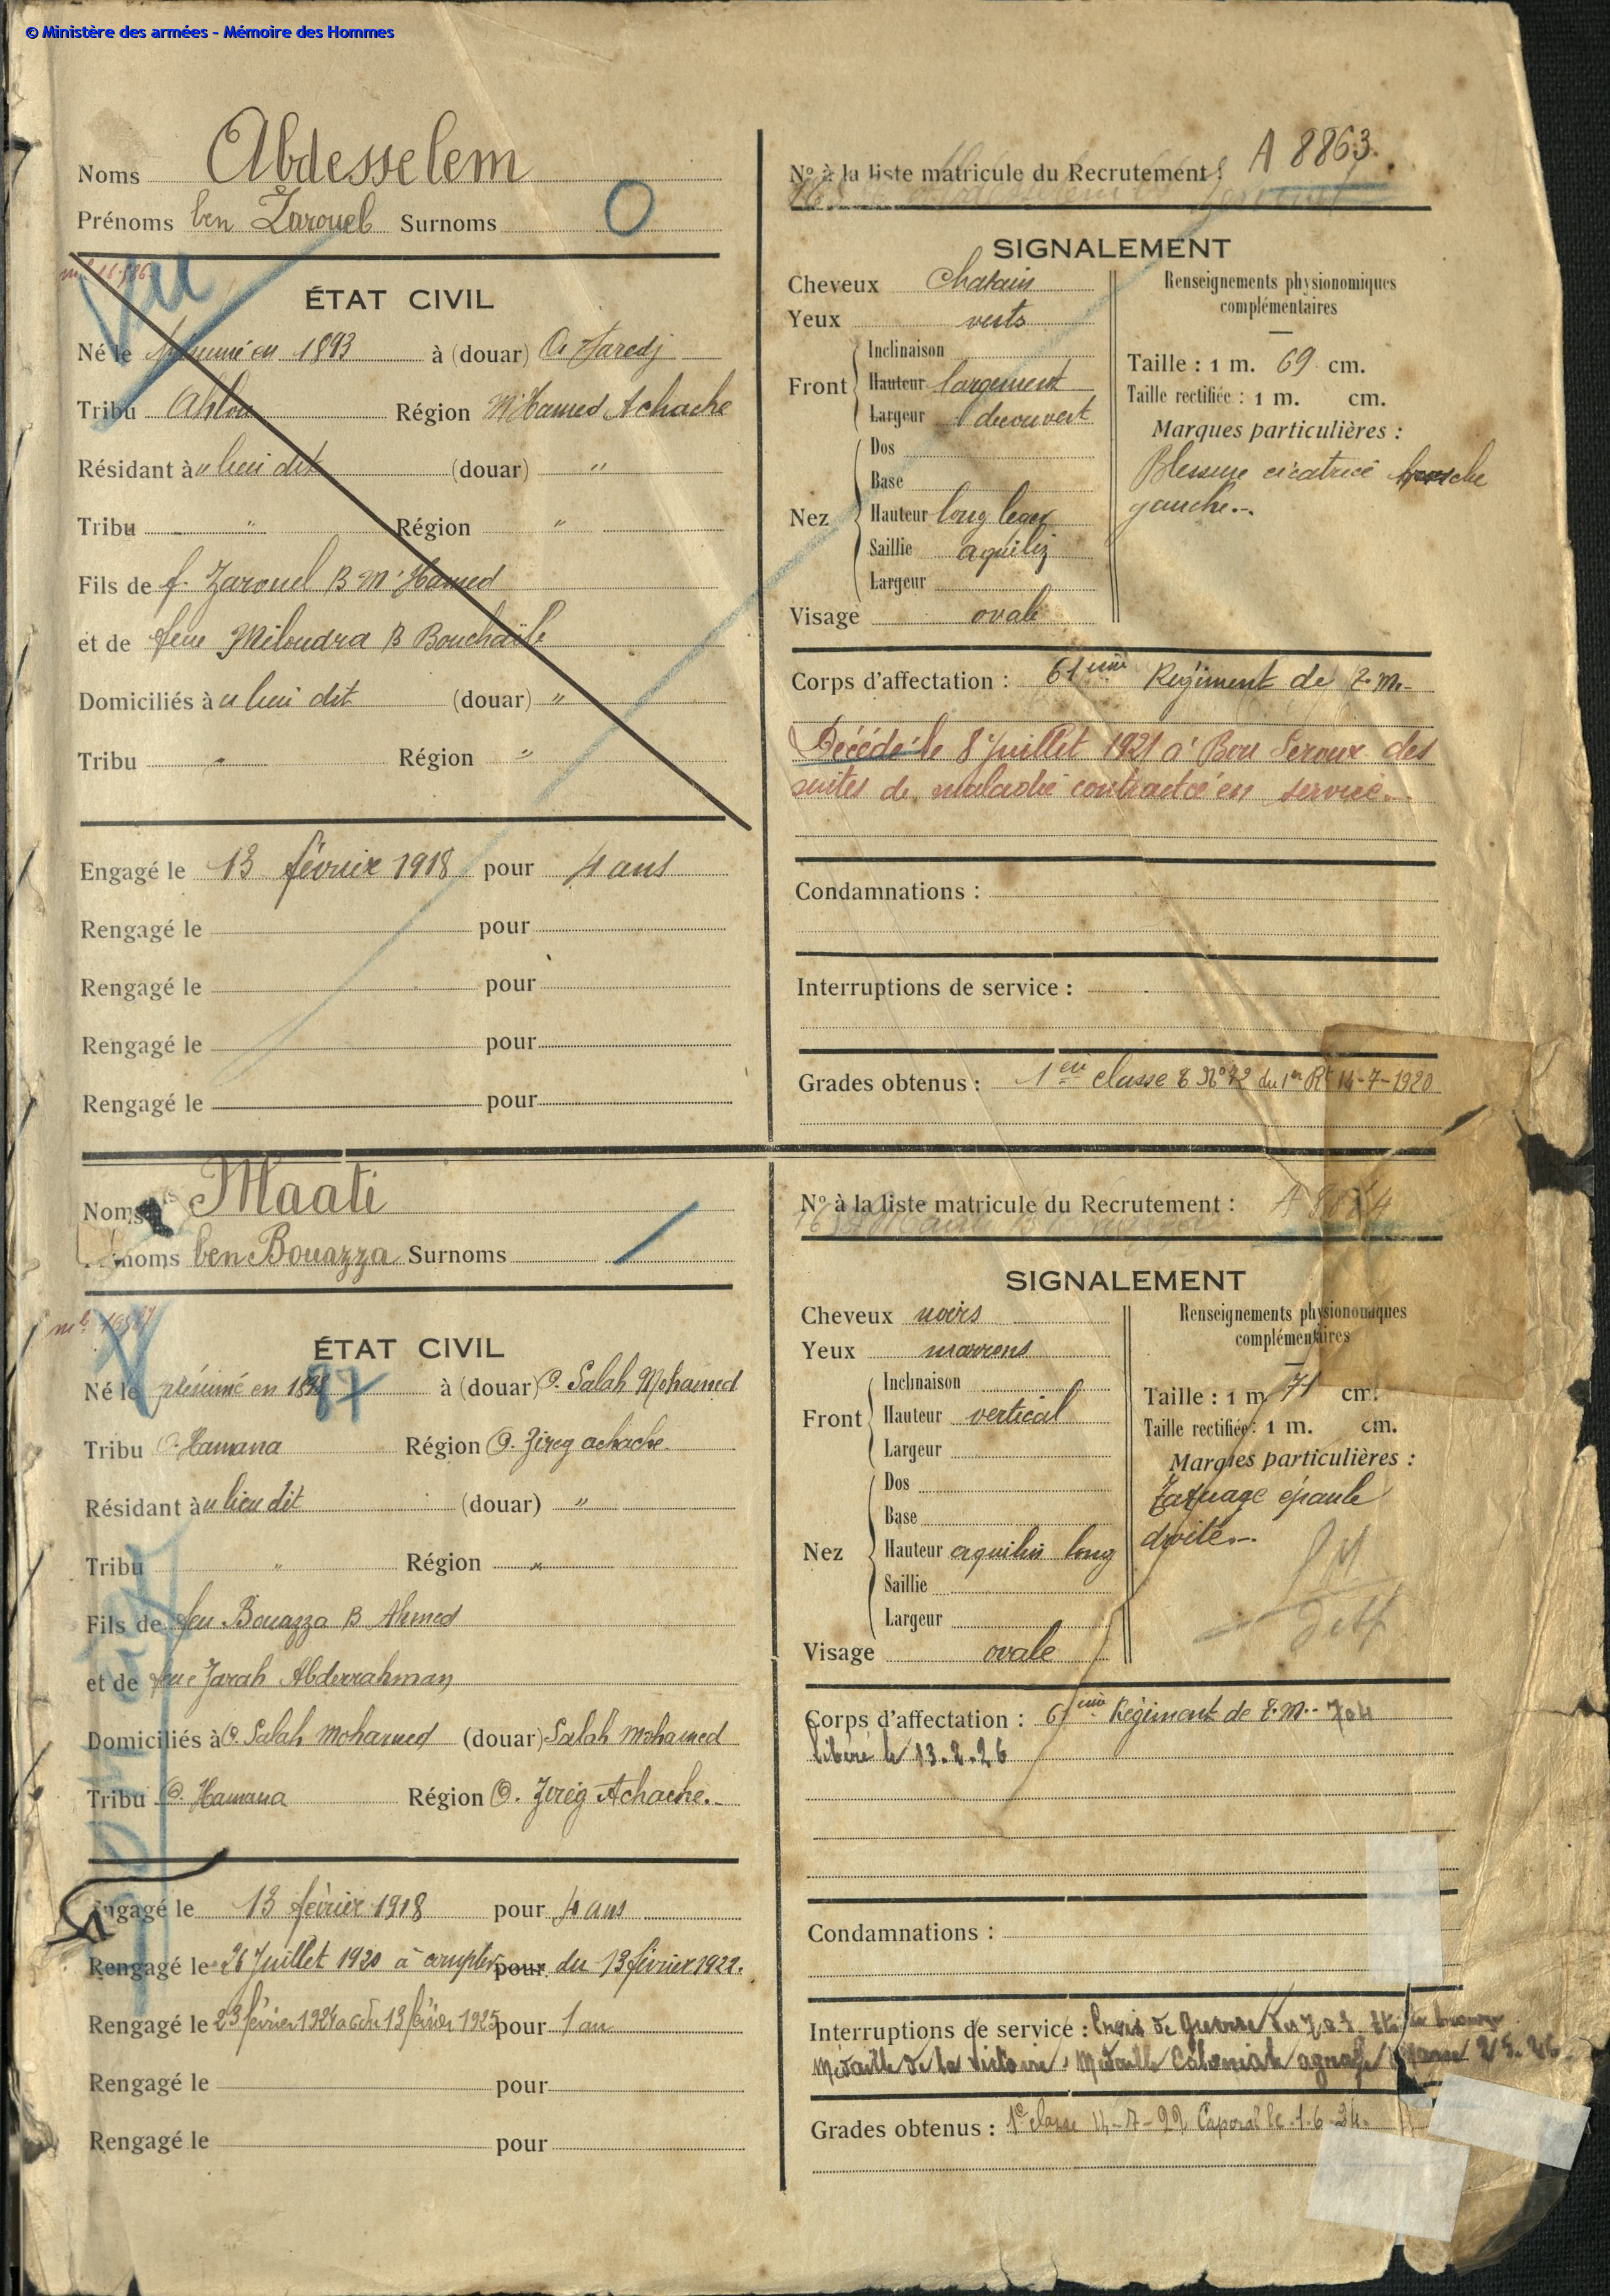
\includegraphics[scale=0.57]{Images/exemplemat2.jpeg}
        \caption[Note d'image]{Un exemple d'un registre matricule du Maroc\footnotemark}
    \label{fig:Mat 2}
    \end{center}
  \end{figure}
  \footnotetext{Source: \url{https://www.memoiredeshommes.sga.defense.gouv.fr/fr/article.php?larub=382&titre=recensement-des-engages-et-appeles-des-anciennes-colonies-francaises}
}

Comme vous pouvez le constater à travers les figures 1.2 et 1.3, les registre matricules sont des formulaires imprimés remplis avec des informations manuscrites. Même si les registres provenant des colonies tendent à être moins riches, ils contiennent le même type d’information que celles qui peuvent être  utiles dans le cadre d’une étude sur l’histoire militaire à grande échelle. On y trouve des indications telles que le corps d’affectation d’un soldat et un événement éventuel comme le décès d’un soldat ou le fait qu’il soit réformé. Elles sont indiquées par un trait noir qui barre l’état civil et l’intégralité de la fiche. Cette pratique est visible dans la figure 1.3 pour le soldat Abdesselem. \\

Étant donné que des unités combattantes de la Grande guerre (nord-africaine, coloniale et métropolitaine) ont également combattus dans  la guerre du Rif, il est possible qu’une quantité importante de registres soit déjà numérisée car ils font partie de la base des fiches matricules de la Grande guerre sur le site Mémoires des hommes. Pour vérifier cela, il serait intéressant de commencer une transcription. Toutes les  fiches matricules des soldats venant du Maroc et certaines d’Algérie sont conservées  au Centre des archives du personnel militaire (CAPM) à Pau. Alors que les fiches matricules des soldats métropolitains qui se trouvent sur les sites des différentes archives départementales sont organisées par classe et non pas par conflit, ce qui rend toute recherche impossible sans la transcription de ces fiches. Pour les soldats de l’armée coloniale (les troupes de marine) et l’armée d'Afrique en Algérie et Tunisie, certains des registres matricules sont numérisés jusqu’à la classe de 1921.\footnote{ Voir : \url{http://anom.archivesnationales.culture.gouv.fr/regmatmil/ 
}.} Le reste des ces registres se trouvent sous forme papier aux Archives nationales d’outre-mer (ANOM) à Aix-en-Provence.\\

\section{Les journaux des marches et opérations}
\urldef\myurl\url{https://www.memoiredeshommes.sga.defense.gouv.fr/fr/article.php%3Flarub%3D2%26titre%3Djournaux-des-unites-engagees-dans-la-premiere-guerre-mondiale}
Les journaux des marches et d'opérations sont les carnets de bord des grandes unités militaires, c'est-à-dire des unités de la taille d'un régiment ou plus. Ces journaux contiennent un large éventail d'informations, allant de la météo et des pertes subites jusqu’au moral des troupes à des moments précis. Il existe des exemples des ces journaux numérisés sur le site du SHD dans la base de données des journaux des unités ayant participées à la Grande Guerre, mais ceux des régiments de marche formés pendant la guerre du Rif, ni d’autres régiments ayant combattu dans cette guerre ne s’y sont pas.\footnote{Voir: \myurl.} Les journaux des marches et opérations (JMO) concernés par mon étude se trouvent actuellement au SHD de Vincennes dans la sous-série 3H des côtes 803 à 1175 qui contient les JMO de la campagne du Rif.\footcites[30]{shd2002} Les JMOs des goums, les unités supplétifs marocaines commandés par des officiers français qui permettraient d'éclairer une histoire encore plus méconnue que celles de troupes coloniales et nord-africaines se trouvent dans les côtes 2375 à 2711 de la même série.\footcites[33]{shd2002}\begin{figure}[h!]
    \begin{center}
      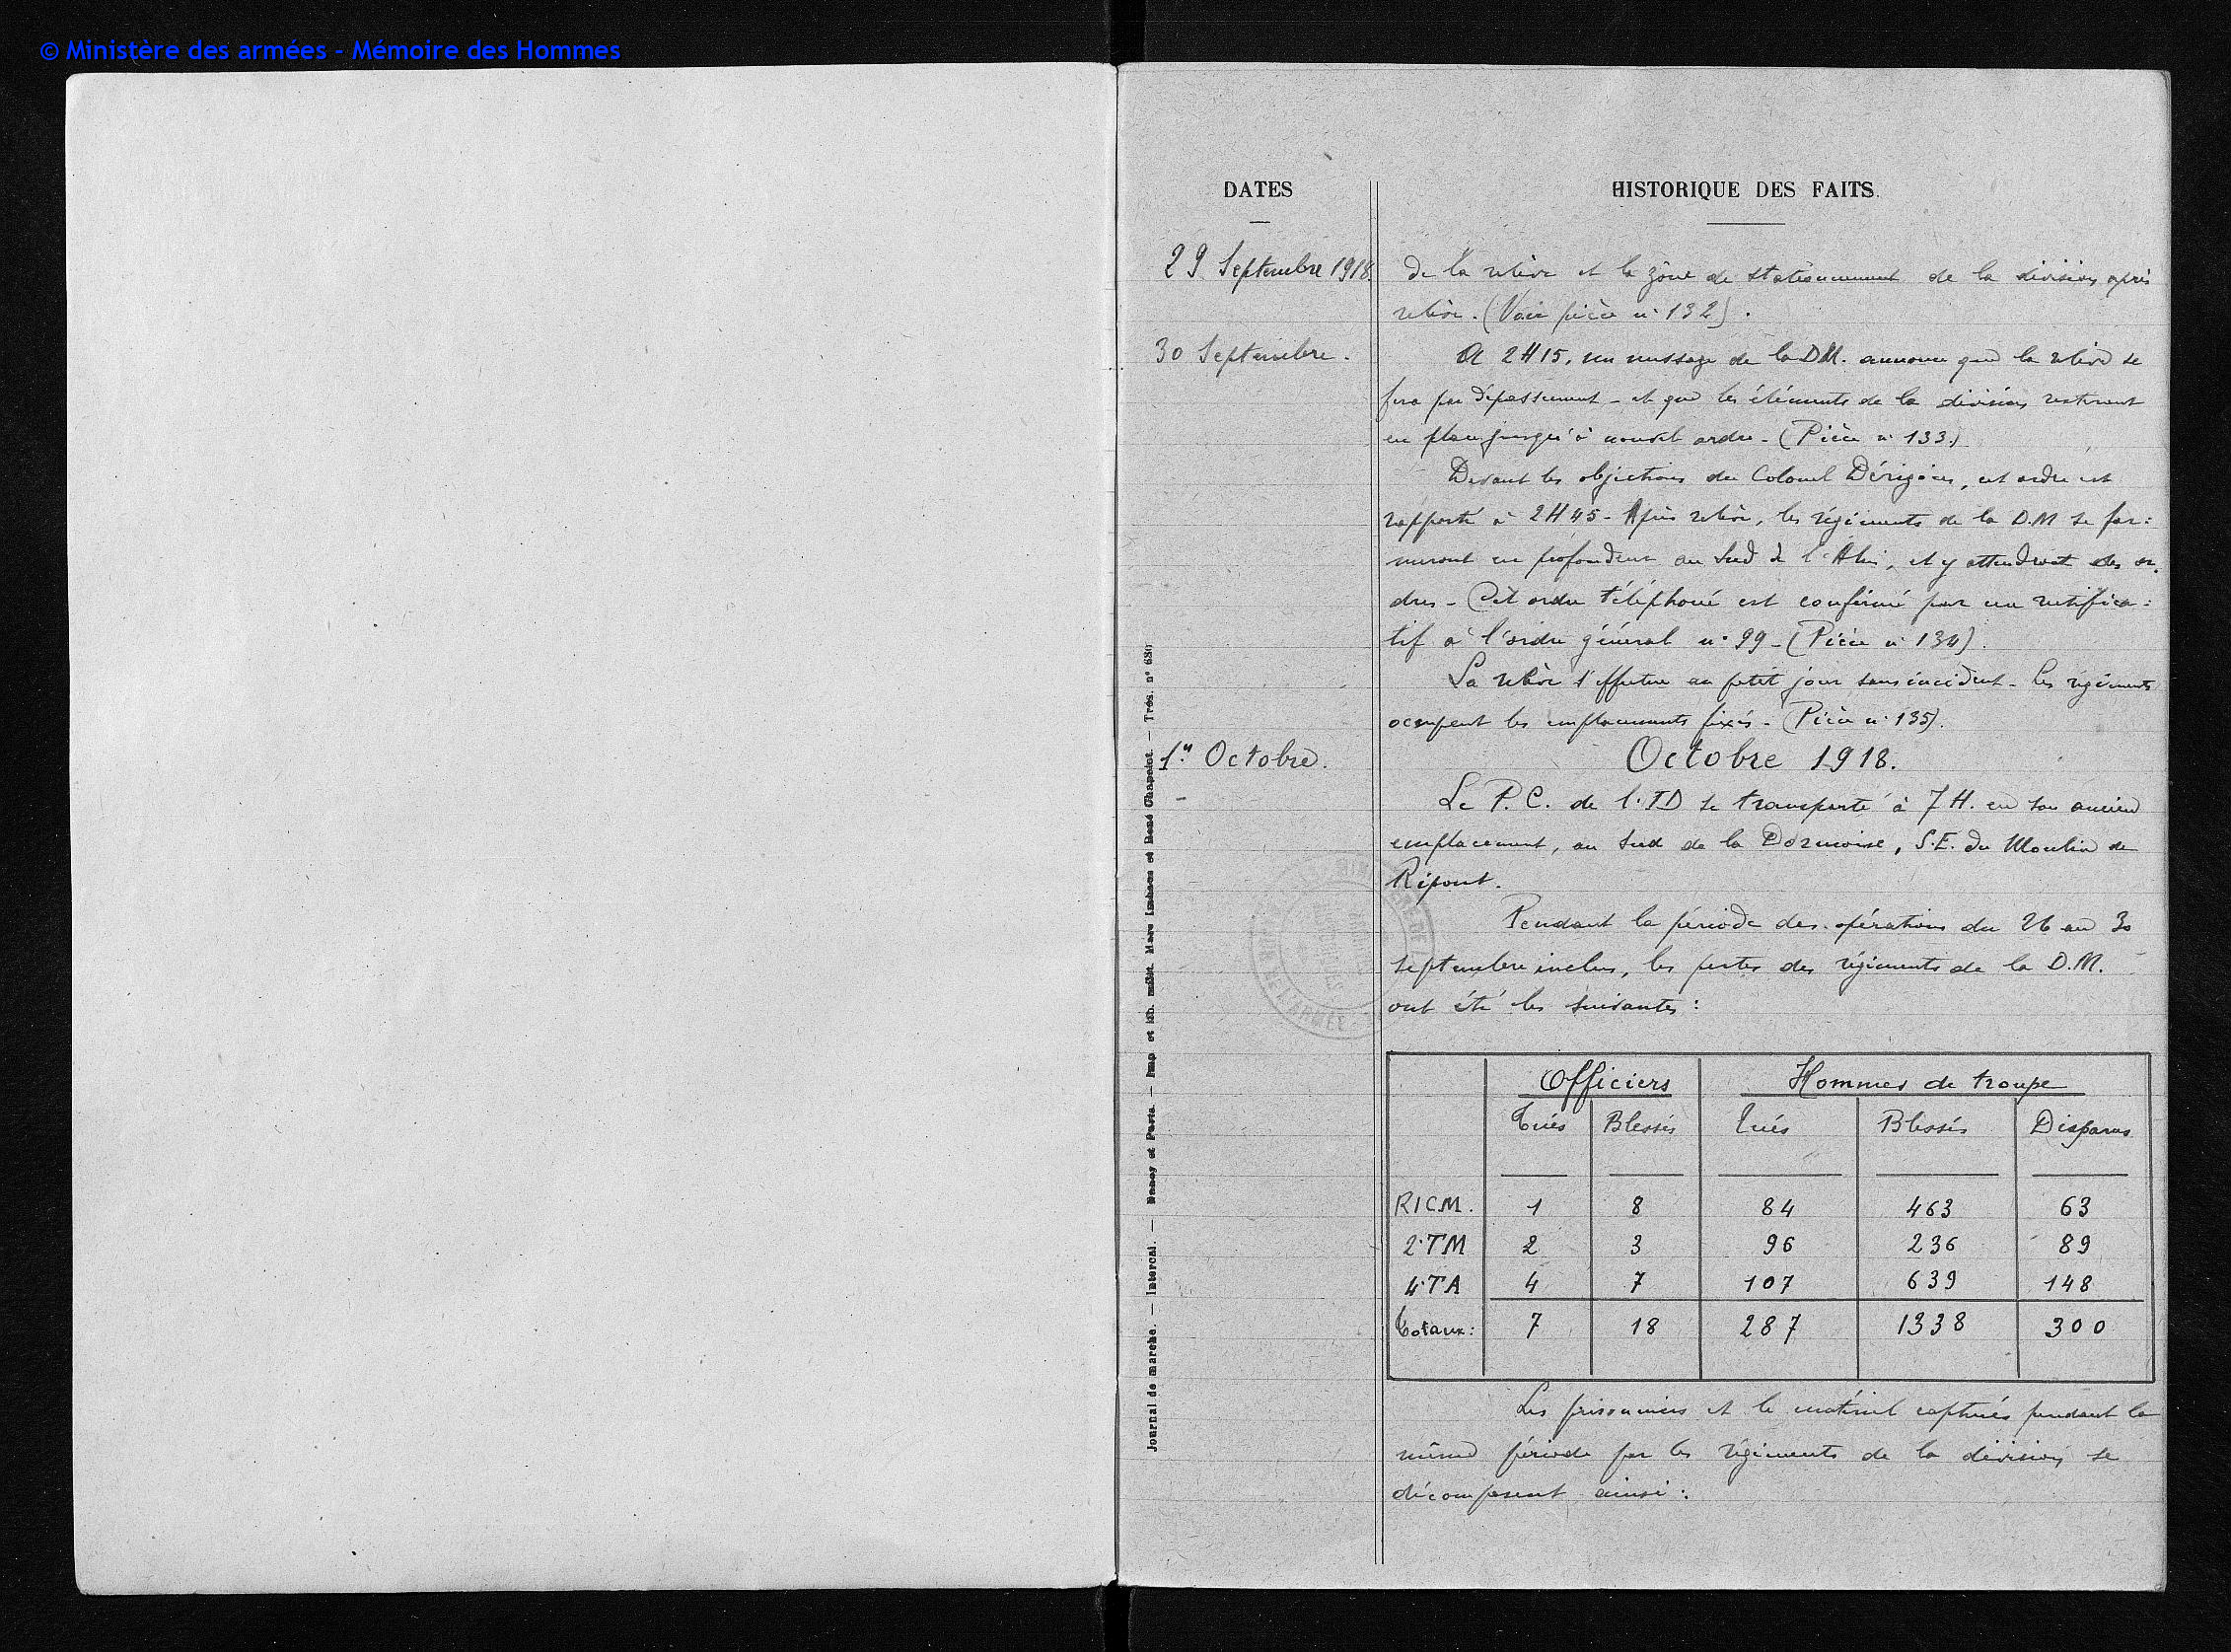
\includegraphics[scale=0.8]{Images/exemplejmo.jpeg}
        \caption[Note d'image]{Un exemple d'un journal des marches et d'opérations\footnotemark}
    \label{fig:JMO}
    \end{center}
  \end{figure}
  \footnotetext{Source: \myurl}

Comme le montre la figure 1.4, ces JMO peuvent constituer un contrôle extrêmement utile de la base de données fournie par le SHD ou de celle créée à partir des fiches matricules transcrites. En bas de page de l’image figure le nombre de pertes subies par la composante d’infanterie de la Division Marocaine  en 1918. Les différents régiments sont indiqués avec leurs pertes par types de soldat (les hommes de troupes et les officiers). En plus de fournir des informations sur les effectifs d’un régiment, les JMOs permettent de faire correspondre les pertes statistiques à des événements militaires tels qu’une offensive ou un siège.\\

\section{Conclusion}
La combinaison de ces trois sources différentes devrait donner un caractère particulier à cette étude. Ce qui ressort de leur utilisation combinée est leur nature équilibrante. En théorie, elles devraient agir comme des garde-fous pour toute conclusion globale que les résultats individuels pourraient suggérer. Couplé d’une lecture de la littérature secondaire et d’une analyse des archives qualitatives, le traitement de sources quantitatives devrait apporter de nouvelles perspectives sur l’histoire de cette guerre. 
\part{Explication des méthodes utilisées}
\chapter{}
\section{Presentation}
Afin de préparer mon travail de M2 et établir une base de référence des données quantitatives, la première étape de ma méthodologie consiste au traitement de la base de données des « Militaires décédés sur les théâtres d'opérations extérieurs (1905-1962) ».  Ensuite je pourrais concevoir un échantillon représentatif de fiches matricules et procéder à une transcription et extraction des données. L’étape finale de la méthodologie serait de vérifier les données présentes avec l’information nichée dans le JMOs pour éviter d'éventuelles analyses anachroniques et essentielles qui pourraient être liées aux méthodes quantitatives. Cette section de mon rapport présentera l'extraction de ma base de données et un aperçu de mes méthodes potentielles pour le traitement des registres matricules. 
\begin{figure}[H]
    \centering
    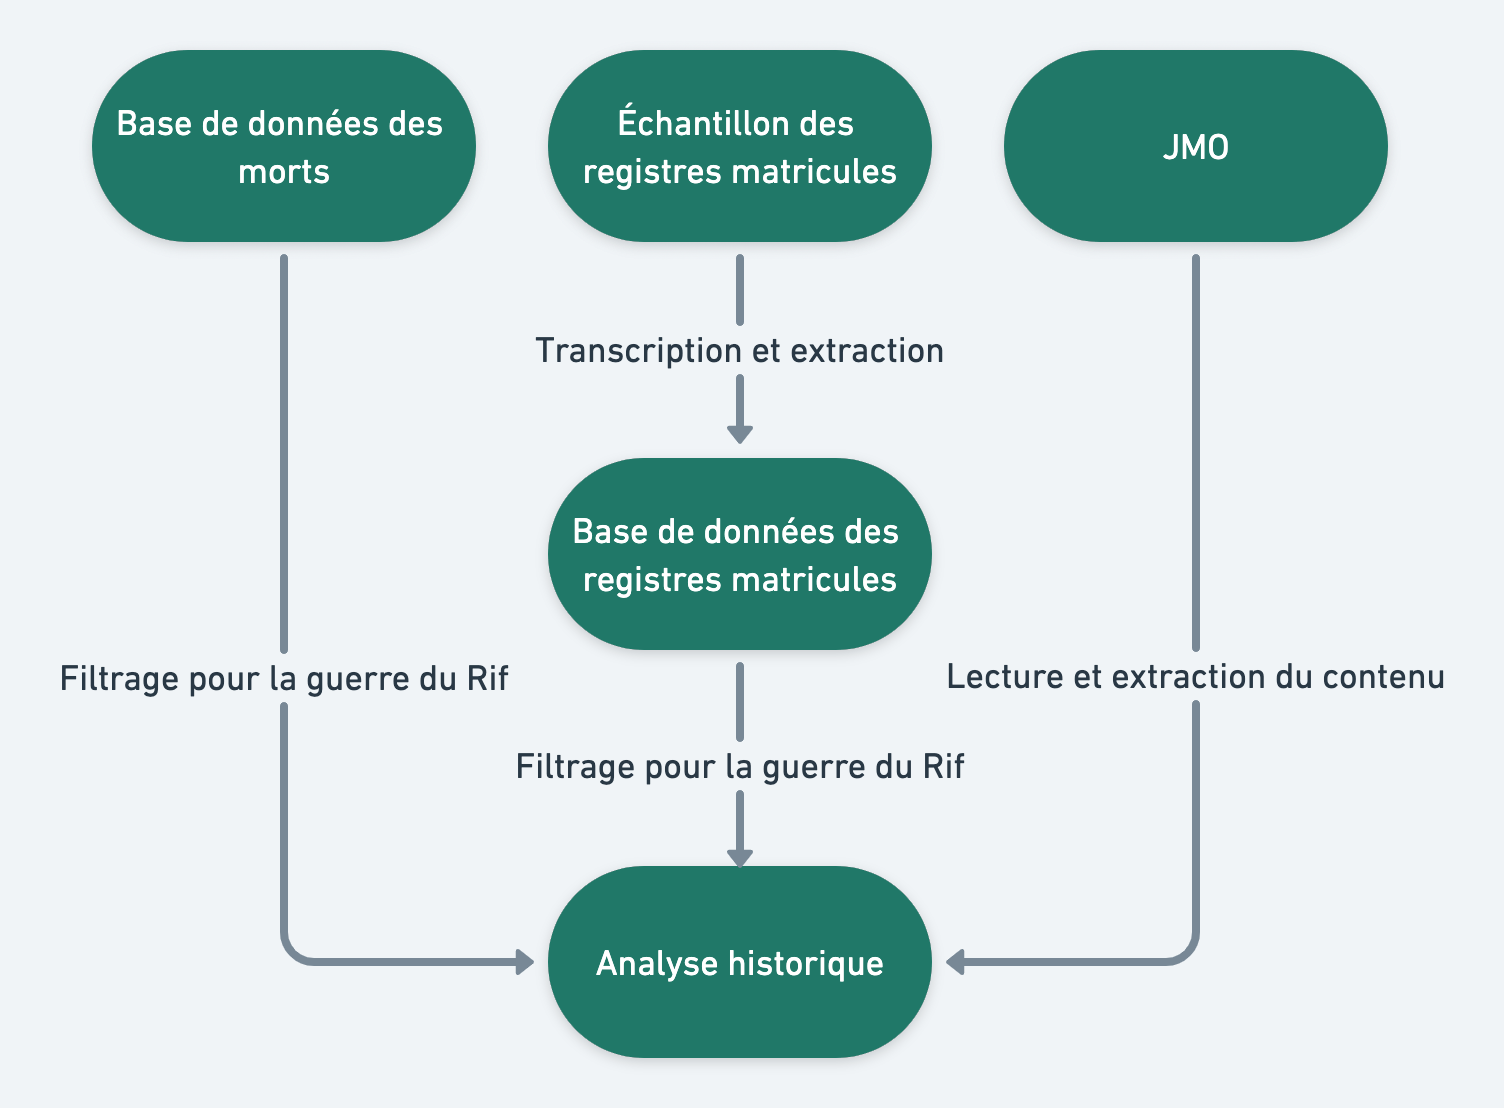
\includegraphics[scale=0.25]{Images/pipeline.png}
    \caption{Organigramme de la méthode}
    \label{fig:Pipeline}
\end{figure}
Enfin, je voudrais attirer l'attention sur un détail que je n'ai pas oublié : les historiens doivent être très prudents lorsqu'ils interprètent des données quantitatives comme une réalité de ce qu'était le passé. De nombreuses études et débats historiographiques ont démontré que la qualité la plus importante pour l'historien quantitatif est l'humilité. Je crois que la méthodologie reflète cette aspiration.

\section{Nettoyage de la base}
Grâce à la disponibilité au format csv de la base de données des morts en opération extérieure, je n'ai pas eu besoin de faire un scrapping du site du SHD. J'ai téléchargé l’intégralité des données directement de ce lien. J'ai ensuite procédé au traitement de la  base « Militaires décédés sur les théâtres d'opérations extérieurs (1905-1962) » avec la librairie \textbf{Pandas} de \textbf{Python}. Après  j'ai filtré la base de données par année et par lieu de décès. La période qui m'intéresse va de janvier 1925 à décembre 1926, la période pendant laquelle la majorité des combats ont eu lieu. Dans la base de données, il y a une colonne pour le pays de décès à partir de laquelle j'ai filtré pour le Maroc. Le script que j'ai utilisé pour filtrer la base de données se trouve sur la \textbf{branch master} dans le dossier \textbf{dbCreation} de mon projet sur \href{https://github.com/the0phil3/projetMemoire}{Github}. Ce travail m'a permis de créer une base de données personnelle des sujets qui m'intéressent.
\begin{figure}[H]
    \centering
    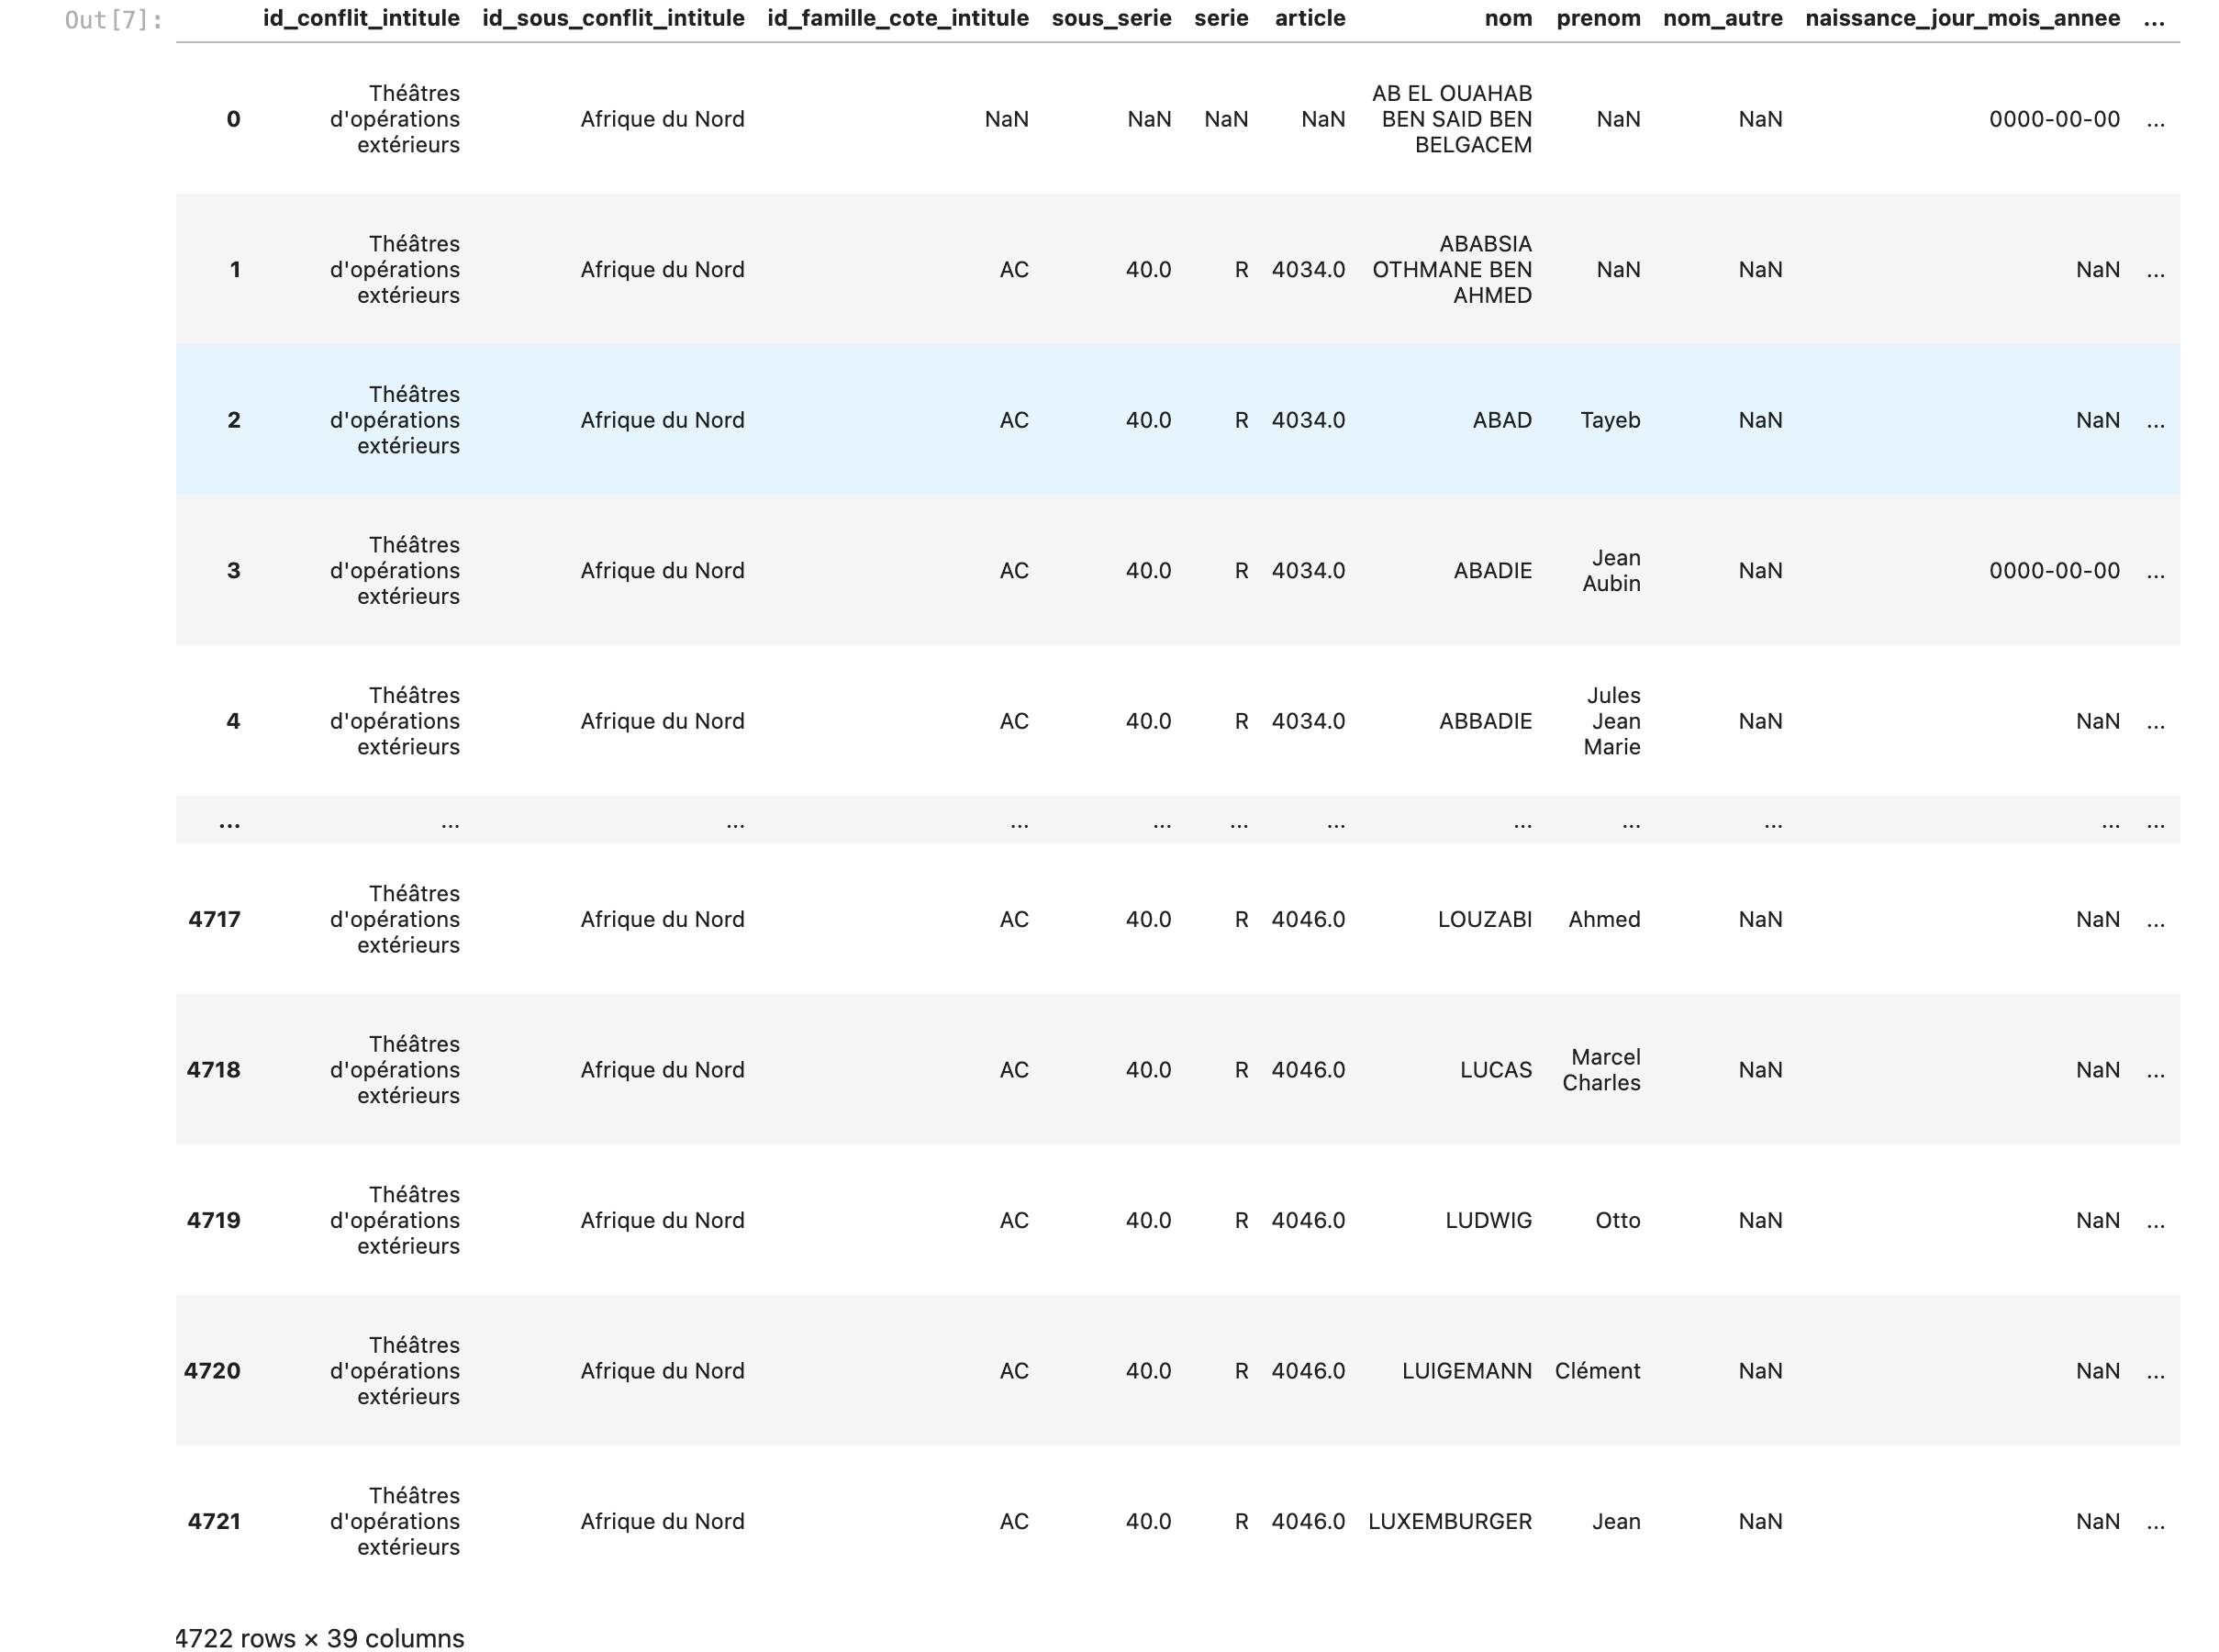
\includegraphics[scale=0.3]{Images/mortsduRif.png}
    \caption{Base de données traitée}
    \label{fig:Base de données}
\end{figure}
Lors de mon premier traitement de cette base de données, j'ai eu comme difficultés que j'ai pu résoudre: \begin{enumerate}
\item Trouver l'origine des données chiffrés 
\item Enlever les doubles des soldats
\item Rendre lisible les dates par \textbf{Pandas}   
\end{enumerate}

L’information disponible sur le site \underline{Mémoire des hommes} au sujet de la base de données concernée est incomplète et m’a obligé à interroger le personnel du SHD pour trouver des réponses. Grâce à un entretien téléphonique que j’ai eu avec un responsable de la Division des Archives des Victimes des Conflits Contemporains du SHD, de Caen, j’ai pu noter que les origines de la base que j’ai déjà traité et comment elle a été constituée : manuellement. Je me suis aussi rendu compte en créant mes premières figures que la base de données n'était pas forcément très propre. J'ai trouvé plusieurs cas d'un double de la même personne. Pour résoudre ce problème j'ai fait un : \begin{verbatim}mortsduRif.drop_duplicates(subset=['nom', 'prenom', 'id_unite_intitule'], 
keep='first')\end{verbatim} Cette manipulation m’a permis d' enlever les doubles des soldats qui existaient. Pour transformer les dates de décès en objet \emph{datetime}, j’ai également fait un : \begin{verbatim} pd.to_datetime(db['deces_annee_mois_jour'], errors='coerce', yearfirst=True, 
format= '%Y/%m/%d')
\end{verbatim}Après une solide analyse de la base de données et après avoir interrogé le personnel du SHD, je suis satisfait de sa qualité et ne peux qu'espérer que les informations qui m'ont été fournies sont exactes. Le décompte final de cette base, après avoir été dédoublée et triée, indique 4679 individus morts avec des caractéristiques variées et un niveau de détail de description assez hétérogène.  

\section{Extraction des registres matricules}
\urldef\maturl\url{https://www.memoiredeshommes.sga.defense.gouv.fr/fr/arkotheque/inventaires/ead_ir_consult.php?ref=20191216_CAPM_BTDA_IR_%E9trangers_Alg%E9rie}
Pour préparer le traitement des registres matricules, j’ai commencé à entraîner un modèle de segmentation et de transcription sur \textbf{eScriptorium} dans le but de transcrire, encoder et extraire des registres matricules les informations relatives aux parcours d’un soldat qui aurait pu combattre pendant la guerre du Rif. Mon corpus potentiel pourrait compter un échantillon du travail numérisation du SHD : « Recensement des engagés et appelés des anciennes colonies françaises - archives matricules (1866-1918) » sur le site \underline{Mémoires des hommes} ainsi qu’un échantillon des fiches nord-africaines de l’ANOM et un tirage des différentes base départementales de fiches matricules.\footnote{Voir : \maturl  ,   \url{http://anom.archivesnationales.culture.gouv.fr/regmatmil/}.} La base d’image sur laquelle je me suis formé, contient pour le Maroc et l'Algérie des classes entières de fiches de plusieurs bureaux de recrutement mais seulement jusqu'à 1919. En total, on y trouve les fiches matricules de plus 8.000 conscrits.\\


 Lors de cet essai, j’ai segmenté mes fiches manuellement avec comme objectif que mon code ALTO puisse être facilement transformé en XML puis en csv. Malheureusement, je n’ai pas réussi à entraîner un modèle de segmentation car je n’en ai pas eu le temps. J’ai eu les mêmes problèmes avec mon modèle de transcription donc pour ce projet j’ai segmenté et transcrit les cinq premiers registres matricule de la côte \textbf{PM B4A17}.  
\begin{figure}[H]
    \centering
    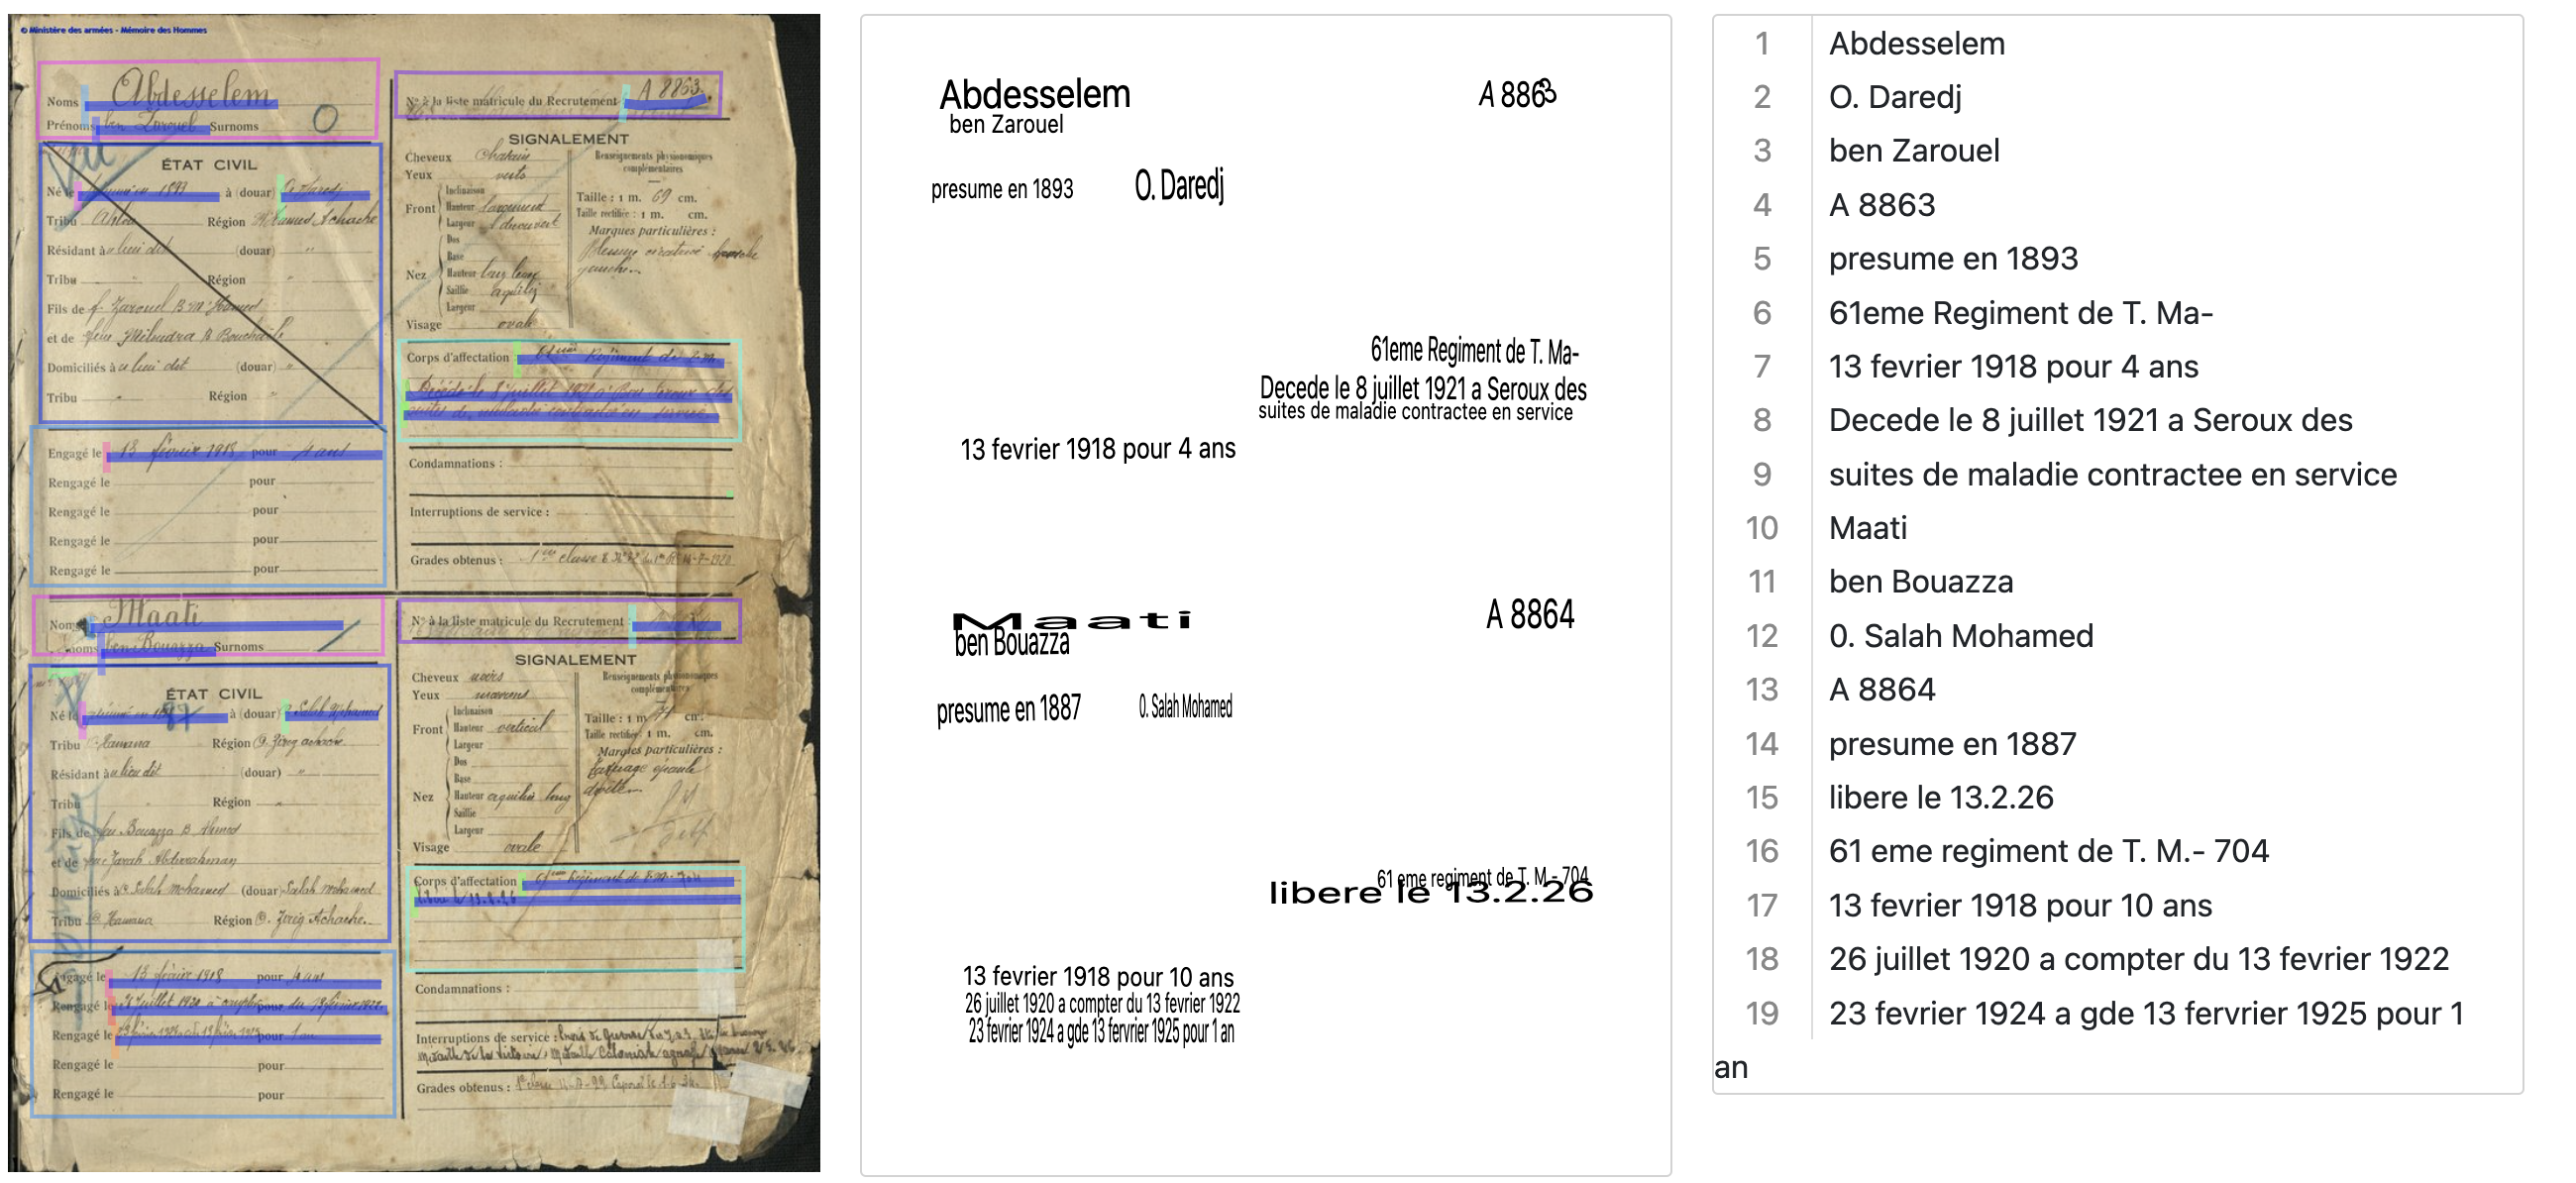
\includegraphics[scale=0.43]{Images/seg.png}
    \caption{Entrainement d'une transcription de matricule Marocain}
    \label{fig:Segmat}
\end{figure}
Ma méthode de segmentation a consisté à créer des régions dans le registre telles que l’état civil, le parcours individuel, le corps d’affection. À l'intérieur de ces régions, j’ai segmenté des lignes spécifiques comme le nom, ou le lieu de naissance. Cette méthode m'a permis d’obtenir des sorties en ALTO qui étaient organisées par contenu. Les fiches matricules originales se trouvent dans le dossier: transcription de mon github. Une fois les transcriptions terminées, j’ai traité ce dossier avec XSLT pour le transformer en XML et ensuite en csv. Avec ces informations stockées dans des fichiers csv, on peut envisager une analyse beaucoup plus claire et puissante des registres matricules. Le but de cet exercice était de me familiariser avec les méthodes de l’HTR afin de préparer le travail d'échantillonnage, de modélisation et de transcription pour l'année prochaine.   
  

\section{Conclusion}
Mon travail de méthodologie de cette année me permet d’avoir un aperçu des résultats que je pourrais obtenir après une étude plus complète. En même temps, il représente une première étape importante dans ma méthodologie, étant donné le manque de conseils reçus sur le plan quantitatif et l'étendue de mes sources qualitatives à traiter. Comme il sera expliqué dans la section suivante, cette étape m'a permis d'effectuer une vérification préliminaire de mes résultats avec d'autres travaux historiques.

\part{Présentation des résultats}
\chapter{}
\section{Presentation}
Les données brutes sur lesquelles se portent  mes résultats se trouvent sur mon  \href{https://github.com/the0phil3/projetMemoire/}{Github} dans le fichier tsv \emph{'mortsduRif'}. Grâce à la quantité de données dont j’ai disposé, j’ai pu procéder à plusieurs manipulations afin d' apporter des explications sur ce qui s’est passé pendant la guerre. La logique qui m’a guidé dans  mes extrapolations a consisté à essayer de pallier au manque de données chiffrées présentées par Max Schiavon dans son ouvrage sur la guerre des français au Rif. Je fais référence à un tableau qu’il y a inclus  indiquant le nombre de morts dûs à  la guerre pendant l’offensive rifaine, entre le printemps et une partie de l’été 1925 : 
\begin{figure}[H]
    \centering
    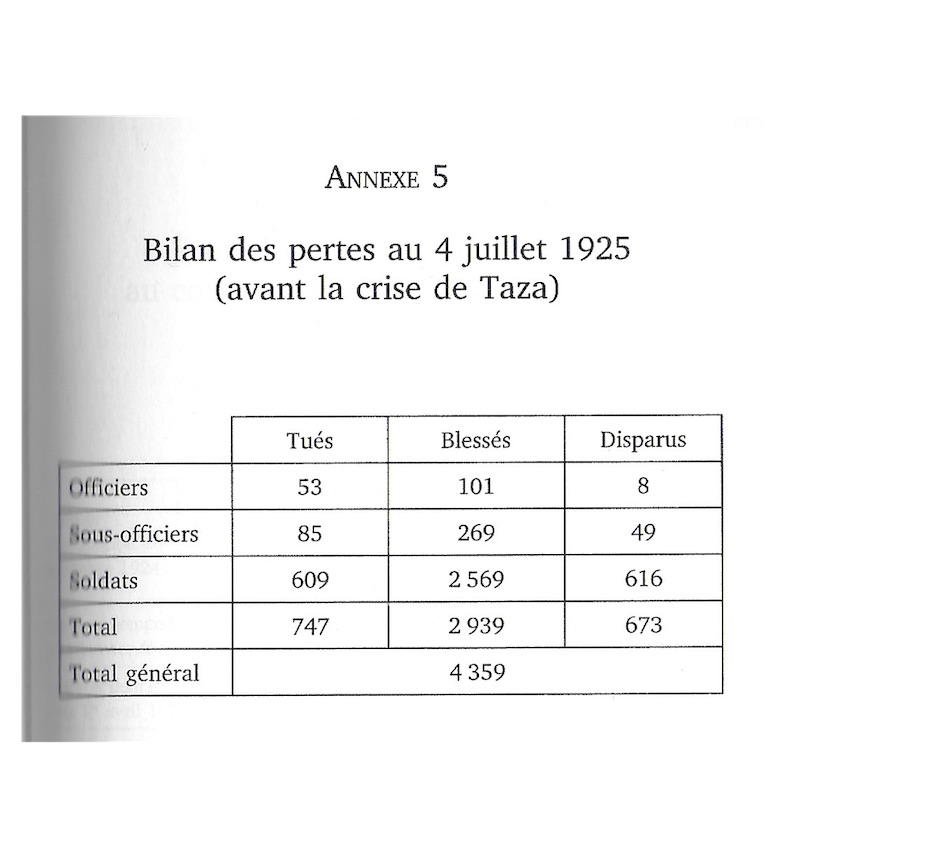
\includegraphics[scale=0.36]{Images/schiavon.jpeg}
    \caption[Note d'image]{Données de Schiavon indiquant les morts avant le 4 juillet 1925\footnotemark}
    \label{fig:Morts Schiavon }
\end{figure} 
\footnotetext{\footcites[309]{schiavon2016}} 
A première vue, il semble que nos données ne coïncident pas  : Schiavon n'enregistre que 747 morts pour les 6 premiers mois de la guerre alors que mes données indiquent 4679 morts pour les deux années de combat. Pourtant, lorsque nous l’on examine en profondeur les dates clés de la guerre et les chiffres fournis par Schiavon et qu’on les compare avec les témoignages des officiers, on constate  que, bien que l'on ne sache pas exactement où Schiavon a recueilli ses données, les deux sont à priori cohérents. Mes résultats se concentrent sur trois domaines
: \begin{enumerate}
    \item les dates
    \item les lieux 
    \item les régiments
\end{enumerate} 

\section{Les dates}
En filtrant pour les dates de la guerre durant lesquelles il y a eu le plus de pertes françaises, j’ai cherché à établir une chronologie des pertes afin de les comparer avec l’historiographie et toute éventuelle informations que les JMOs ou registres matricules pourraient apporter. Les résultats que j’ai obtenus en calculant les jours où il y a eu  le plus de pertes sont présentés dans la figure 3.2. Ce qui est frappant dans cette figure est la prédominance de la période 1925 à 1926 dans son caractère meurtrier. Cette tendance est commune au reste des résultats pour les dates, qui se trouvent en annexe.\footnote{Voir annexe : \ref{fig:Dates 2}}
\begin{figure}[H]
    \centering
    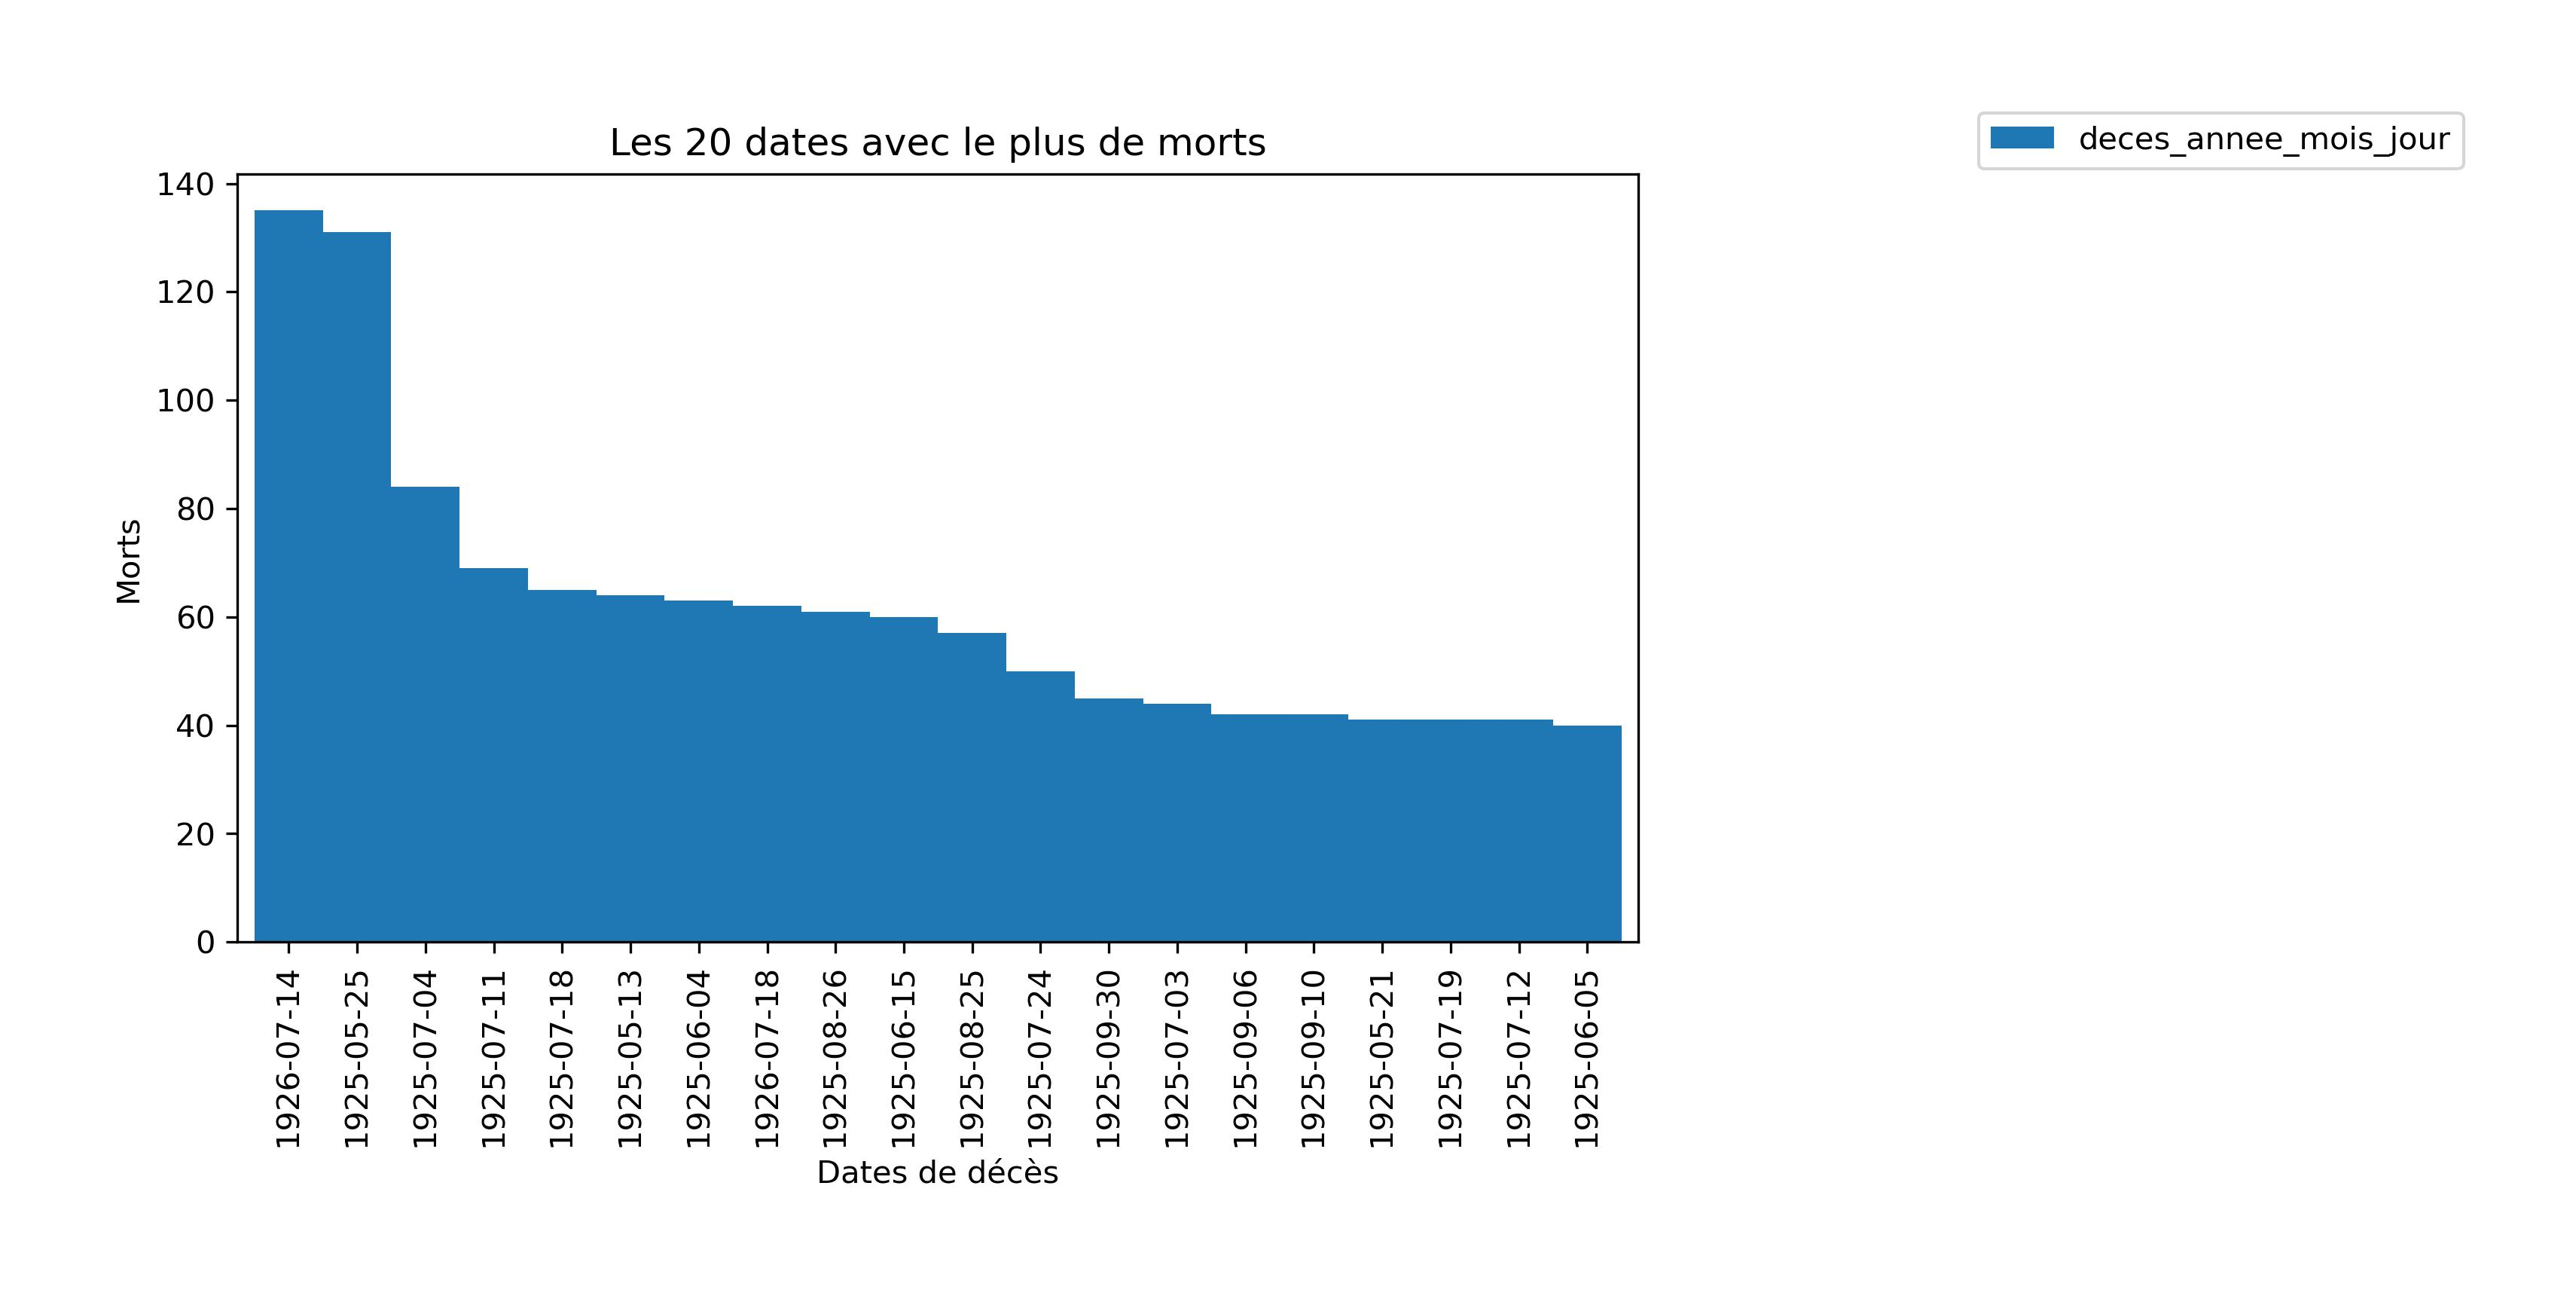
\includegraphics[scale=0.58]{Images/20dates.jpg}
    \caption{Les 20 jours avec le plus de pertes pour l'armée française}
    \label{fig:Morts par jour}
\end{figure}
En outre, la date qui enregistre le plus grand nombre de morts, le 14 juillet 1926, est curieuse car il s’agit d’ une valeur isolée dans la tendance. Lorsqu’on examine les récits de l’offensive française de 1926, on comprend pourquoi cette journée a été si meurtrière. Dans le témoignage du jeune lieutenant Joubert, la préface du général Dufieux décrit l’attaque de « la grande Tache de Taza » où l’avant-garde de la brigade de Ganay sous le commandant Croizé résiste  aux Rifains.\footcites[7]{joubert1927} Le commandant Croizé meurt quatre jours plus tard lors de la même offensive. Par ailleurs, si l’on essaie  de situer mes données dans la chronologie de Schiavon, on comprend pourquoi son tableau contient si peu de morts. Il correspond à des dates antérieures à la fin de la période dite " Héroïque " de la guerre lorsque l'armée française n'est pas encore sollicitée jusqu'au point de rupture.\footcites[143]{schiavon2016}La lecture que fait Schiavon de ses propres données est révélatrice pour mon comparatif car il présente lui-même leurs propres insuffisances. Il écrit qu’ à ces chiffres de 1 005 morts, il faut ajouter 997 disparus et 478 morts par maladie, accident ou suicide, ce qui porte le décompte à environ 2 480 morts.\footcites[145]{schiavon2016} Un chiffre qui correspond mieux aux relevés du SHD compilés 100 ans après ce conflit. .
\section{Les lieux}
Les informations que la base de données de morts fournit pour les lieux de décès sont également en accord avec les  tendances historiographiques de la guerre du Rif. La figure 3.3 donne un aperçu de mes résultats pour le calcul des lieux avec le plus de pertes. Le reste de figures se trouvent dans les annexes.\begin{figure}[H]
    \centering
    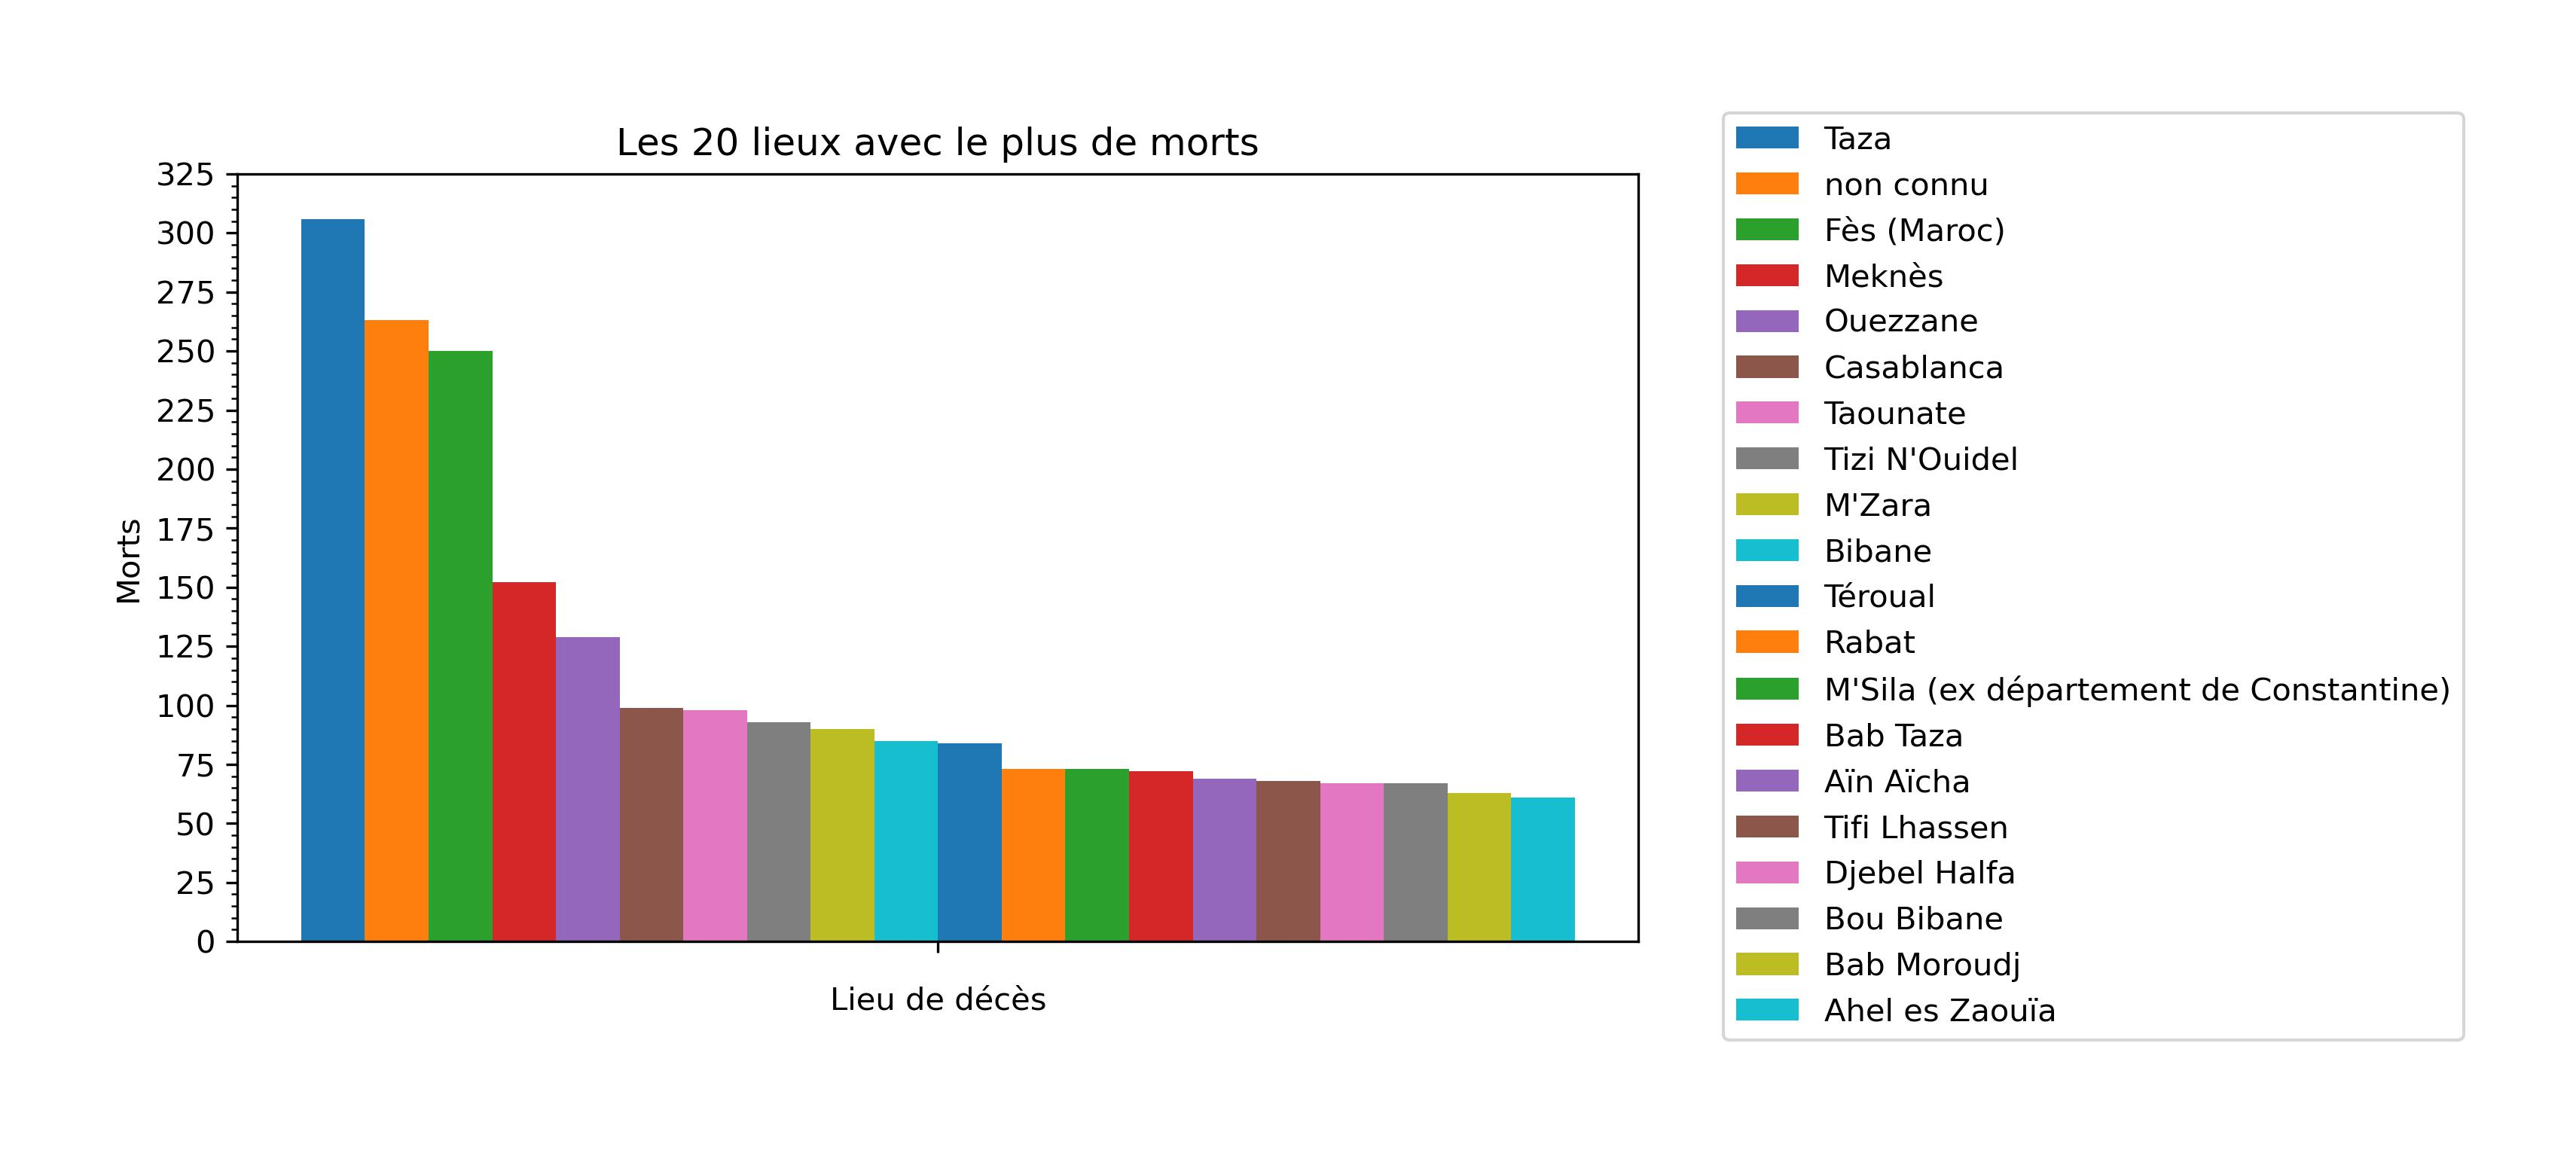
\includegraphics[scale=0.5]{Images/20places.jpg}
    \caption{Les 20 lieux avec le plus de pertes pour l'armée française}
    \label{fig:Morts par lieux}
\end{figure} 
La prédominance de lieux comme Taza, Ouezzane et Meknès dans la partie supérieure de la figure correspond précisément aux récits dominants du conflit. Le témoignage de Walter B. Harris, spécialiste du Maroc, contemporain de la guerre, indique que les combats les plus violents de la campagne de 1925 ont eu lieu sur la ligne entre Taza et Ouezzane.\footcites[226]{harris1925} L’analyse de Schiavon est tout à fait en accord avec ce constat. 
\section{Les régiments}
En ce qui concerne les régiments qui ont subi le plus de pertes, la question de la conformité des résultats à l'état actuel de l'historiographie est plus complexe. Ceci est dû au manque d’études sur le sujet. En dehors de  Schiavon, qui soutient que les soldats métropolitains et officiers subalternes ont subi une plus grande proportion de pertes dans leurs effectifs que les soldats nord-africains, très peu d’études ont été consacrées aux différentes composantes des armées français qui y ont participé.\footcites[145]{schiavon2016} D'après mes résultats, on peut constater que les régiments de la légion étrangère composés de soldats non-français mais non issus l’empire, ont un place importante. Mais les différents régiments de tirailleurs occupent aussi une place de choix en haut du classement.
\begin{figure}[H]
    \centering
    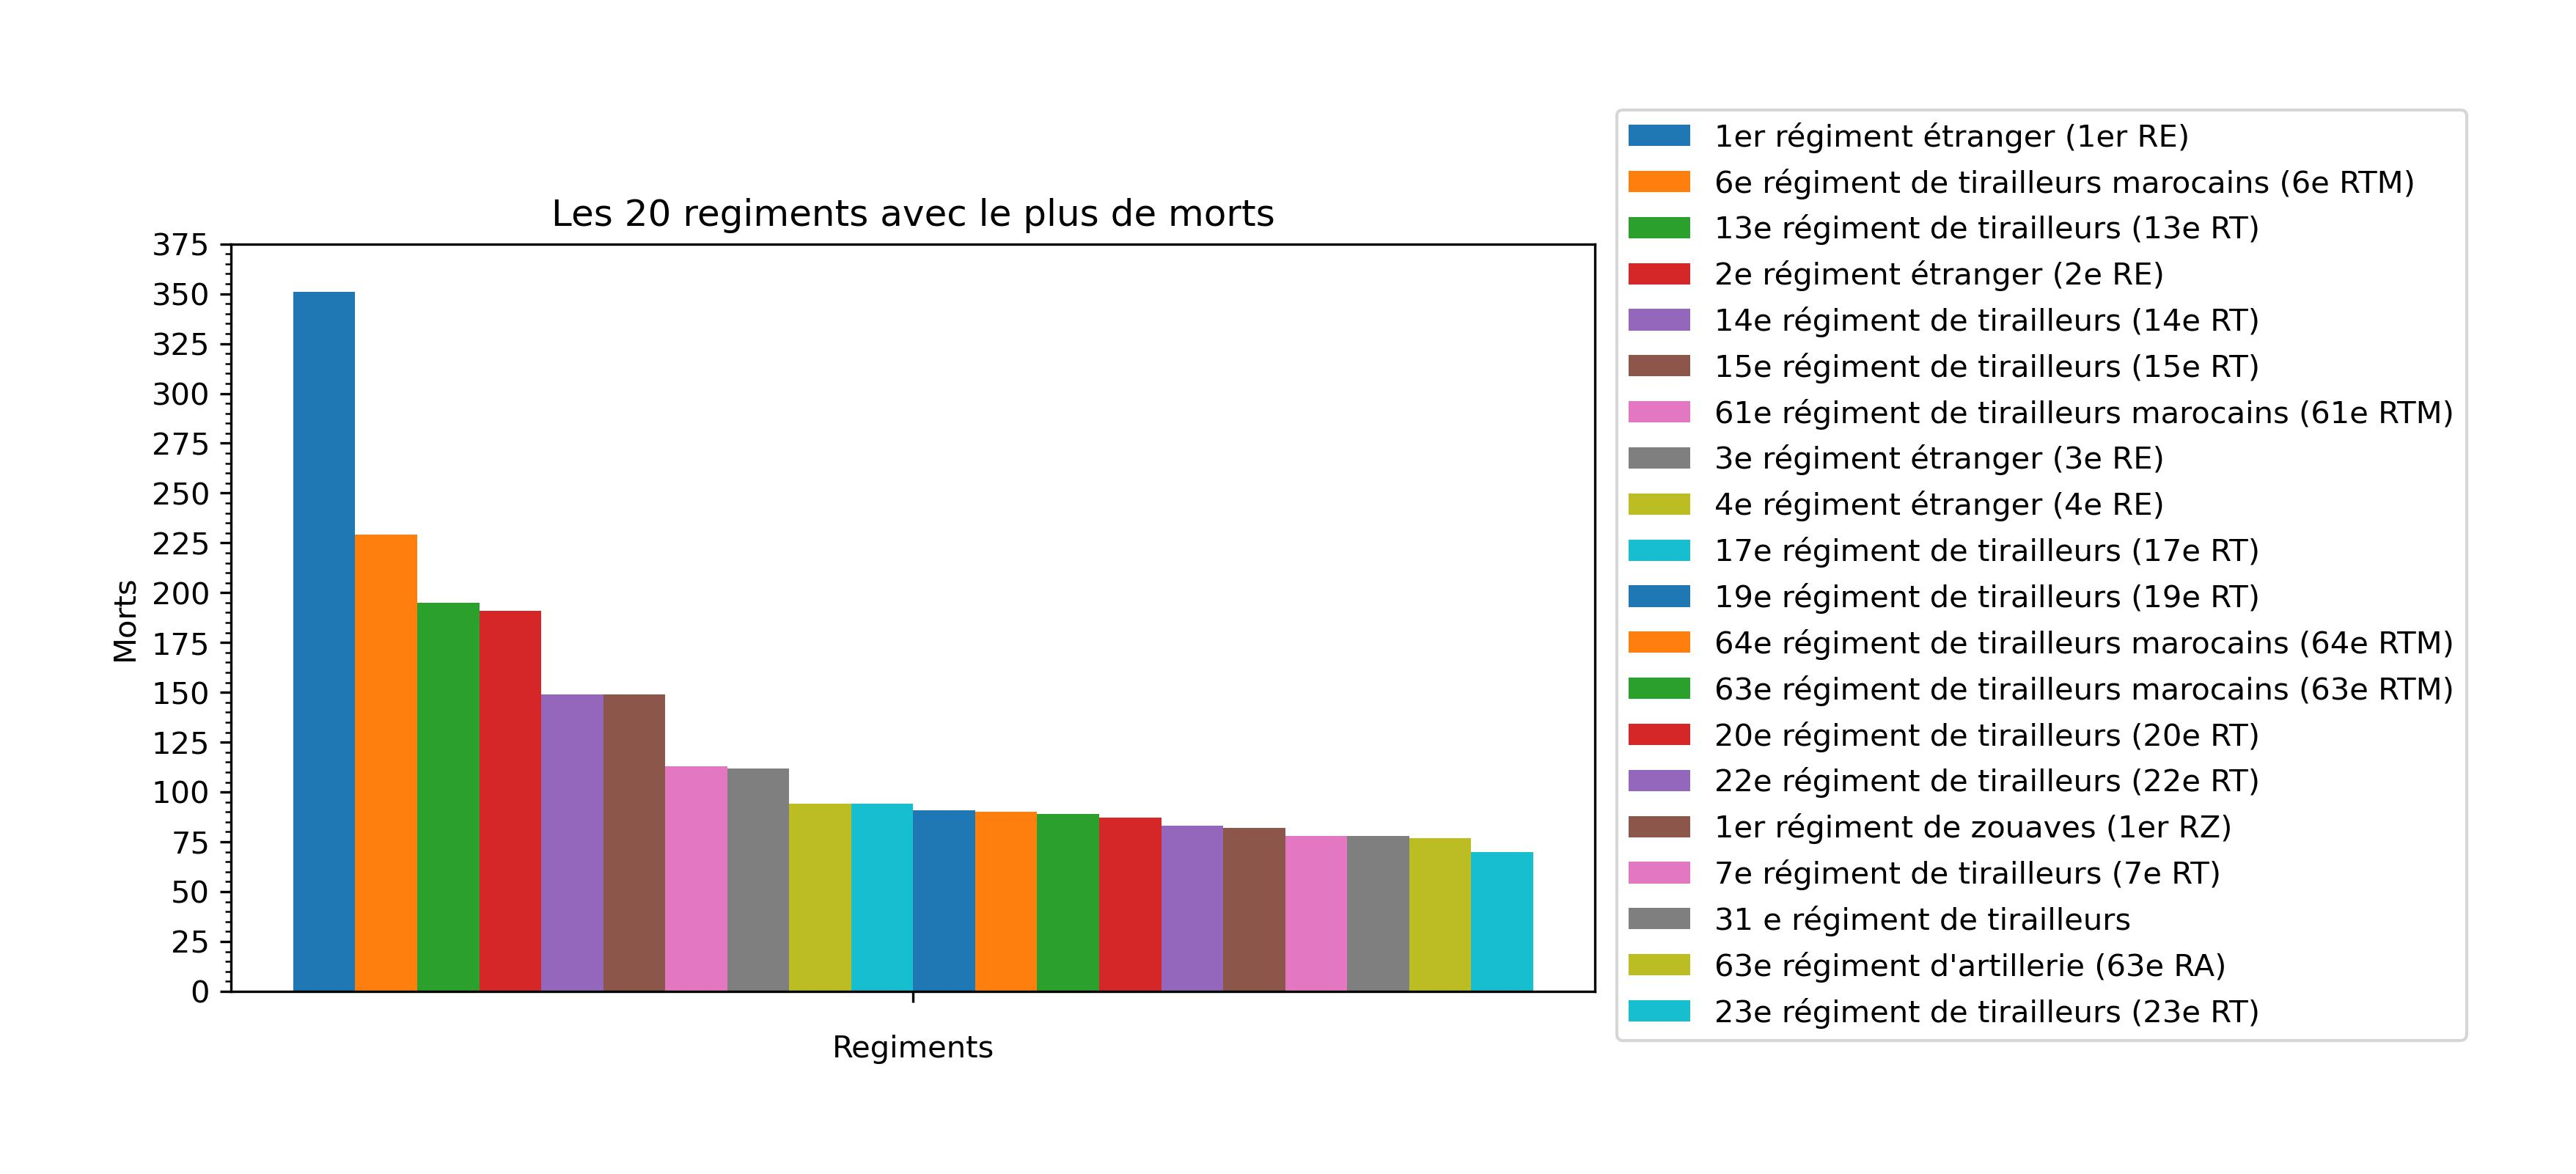
\includegraphics[scale=0.6]{Images/20regiments.jpg}
    \caption{Les 20 régiments avec le plus de pertes pour l'armée française}
    \label{fig:Morts par régiments}
\end{figure} 
 En observant l’ensemble des figures jointes dans l'annexe, il est clair que les régiments nord-africains sont majoritairement représentés dans les régiments ayant subi les plus pertes. Une explication potentielle de la présence des régiments de la légion en haut du classement des pertes pourrait venir de leur réputation de troupes d’élites. Dans l’ensemble, ces résultats restent difficiles à expliquer et contextualiser sans une idée claire du nombre de troupes préparées pour la campagne par régiment. Cette information pourrait se trouver dans les JMOs.

\section{Conclusion}
Bien que certains éléments importants manquent, l’ensemble de mes résultats sont en accord avec le faible éclairage  historiographique existant. Cependant, le résultat est un indicateur positif de la qualité des données disponibles sur le SHD. Cela ne signifie pas pour autant que d'autres travaux historiques doivent être négligés ou que ma méthodologie ne doit pas être remise en question. La taille  de la base de données montre clairement qu'il y a beaucoup plus de latitude pour analyser, comparer et traiter les caractéristiques des soldats qui y sont enregistrés.   

\part*{Conclusion}
\addcontentsline{toc}{part}{Conclusion}
\markboth{Conclusion}{Conclusion} 
Mon rapport constitue un premier pas vers une étude compréhensive et raisonnée de la guerre du Rif. En ce qui concerne mes sources, ma méthodologie et mes résultats, mon travail a consisté à essayer de développer une méthode qui pourrait être utilisée pour tirer des conclusions pertinentes par rapport aux enjeux d’aujourd’hui avec les outils du moment.\\ 

Mes sources forment la colonne verticale de mon mini-mémoire et constitueront la base de mon mémoire final. Fondamentalement, je suis satisfait de leur capacité à se complémenter mutuellement. Cependant, je reconnais que l'utilisation de deux de mes trois sources primaires (les registres matricules et les JMOs) soulève des questions quant à leur caractère pratique. Les problèmes d’échantillonnage des registres matricules et l'entraînement des modèles qui vont les transcrire n’ont pas encore trouvé de réponse. Ils méritent que je m’y attarde au plus vite afin de mieux préparer mes démarches pour l'année prochaine. D’autre part, le fait que je n’ai pas encore eu le temps de vérifier l’état des JMOs de la guerre du Rif le place en tête de mes priorités. Une fois que ces deux points auront été réglés,  je pourrai procéder à mes recherches de manière méthodique.\\ 

Dans sa globalité, ma méthodologie prend en compte les complexités du terrain et tente d’y répondre  sous un maximum d’angles. Cela peut entraîner des contraintes de temps et des difficultés de collecte et le traitement de données mais c’ est nécessaire pour que je puisse garder un lien fort entre mes archives qualitatives et quantitatives. Le but de ce lien étant de ne pas se limiter à l’une de ces deux catégories.\\ 

Les résultats que j’ai pu montrer ont servi pour éclairer des détails intéressants sur le déroulement des combats. Il n’y avait que peu ou pas de valeurs aberrantes dans mes résultats, même en tenant compte de l’absence  d’un objet de comparaison pour certaines données. Cependant, je reconnais que l’extrapolation et le traitement de la base de données des décès auraient pu être plus approfondis.  Plus précisément, du côté du code, j'aurais pu rechercher davantage de relations entre les différentes caractéristiques des soldats morts  pendant cette guerre. J’en suis conscient et je sais que je dois encore effectuer un travail d'apprentissage des modèles de régression de \textbf{scikit-learn}et d’approfondissement de mes compétences avec \\textbf{pandas} en \textbf{python}.\\ 




% annexes
\appendix
\part*{Annexes}
\addcontentsline{toc}{part}{Annexes}
\pagestyle{myheadings}
\markboth{Annexes}{Annexes}

Template LaTeX disponible ici : \url{https://github.com/ChartesHN/}.

Tout mon code est disponible ici : \url{https://github.com/the0phil3/projetMemoire/}.

Le moteur de recherche de la base données du SHD : 
\begin{figure}[h]
    \centering
    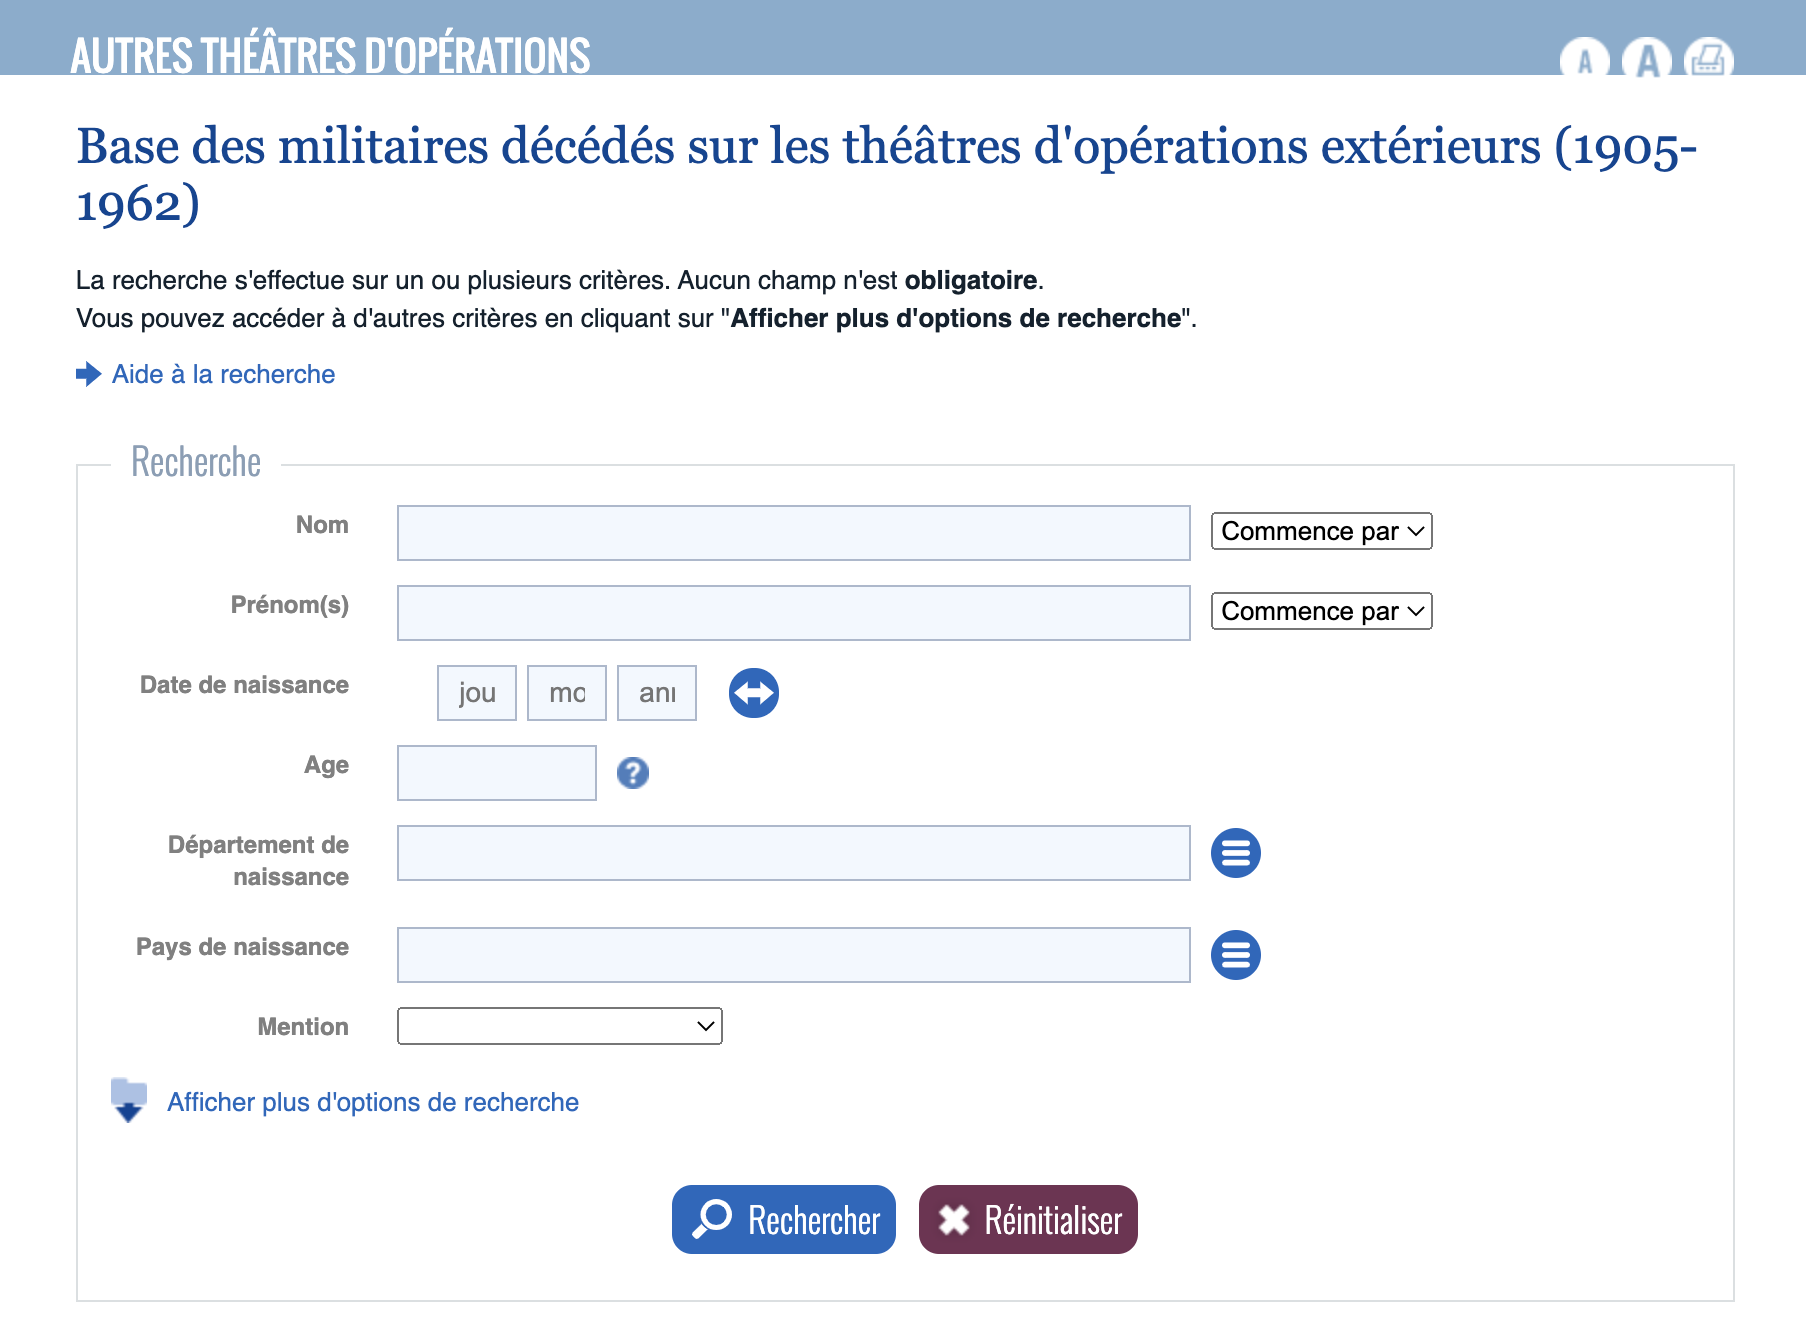
\includegraphics[scale=0.27]{ark1.png}
    \caption{Moteur de recherche simple}
    \label{fig:Arkothèque 1}
\end{figure}
\begin{figure}[h]
    \centering
    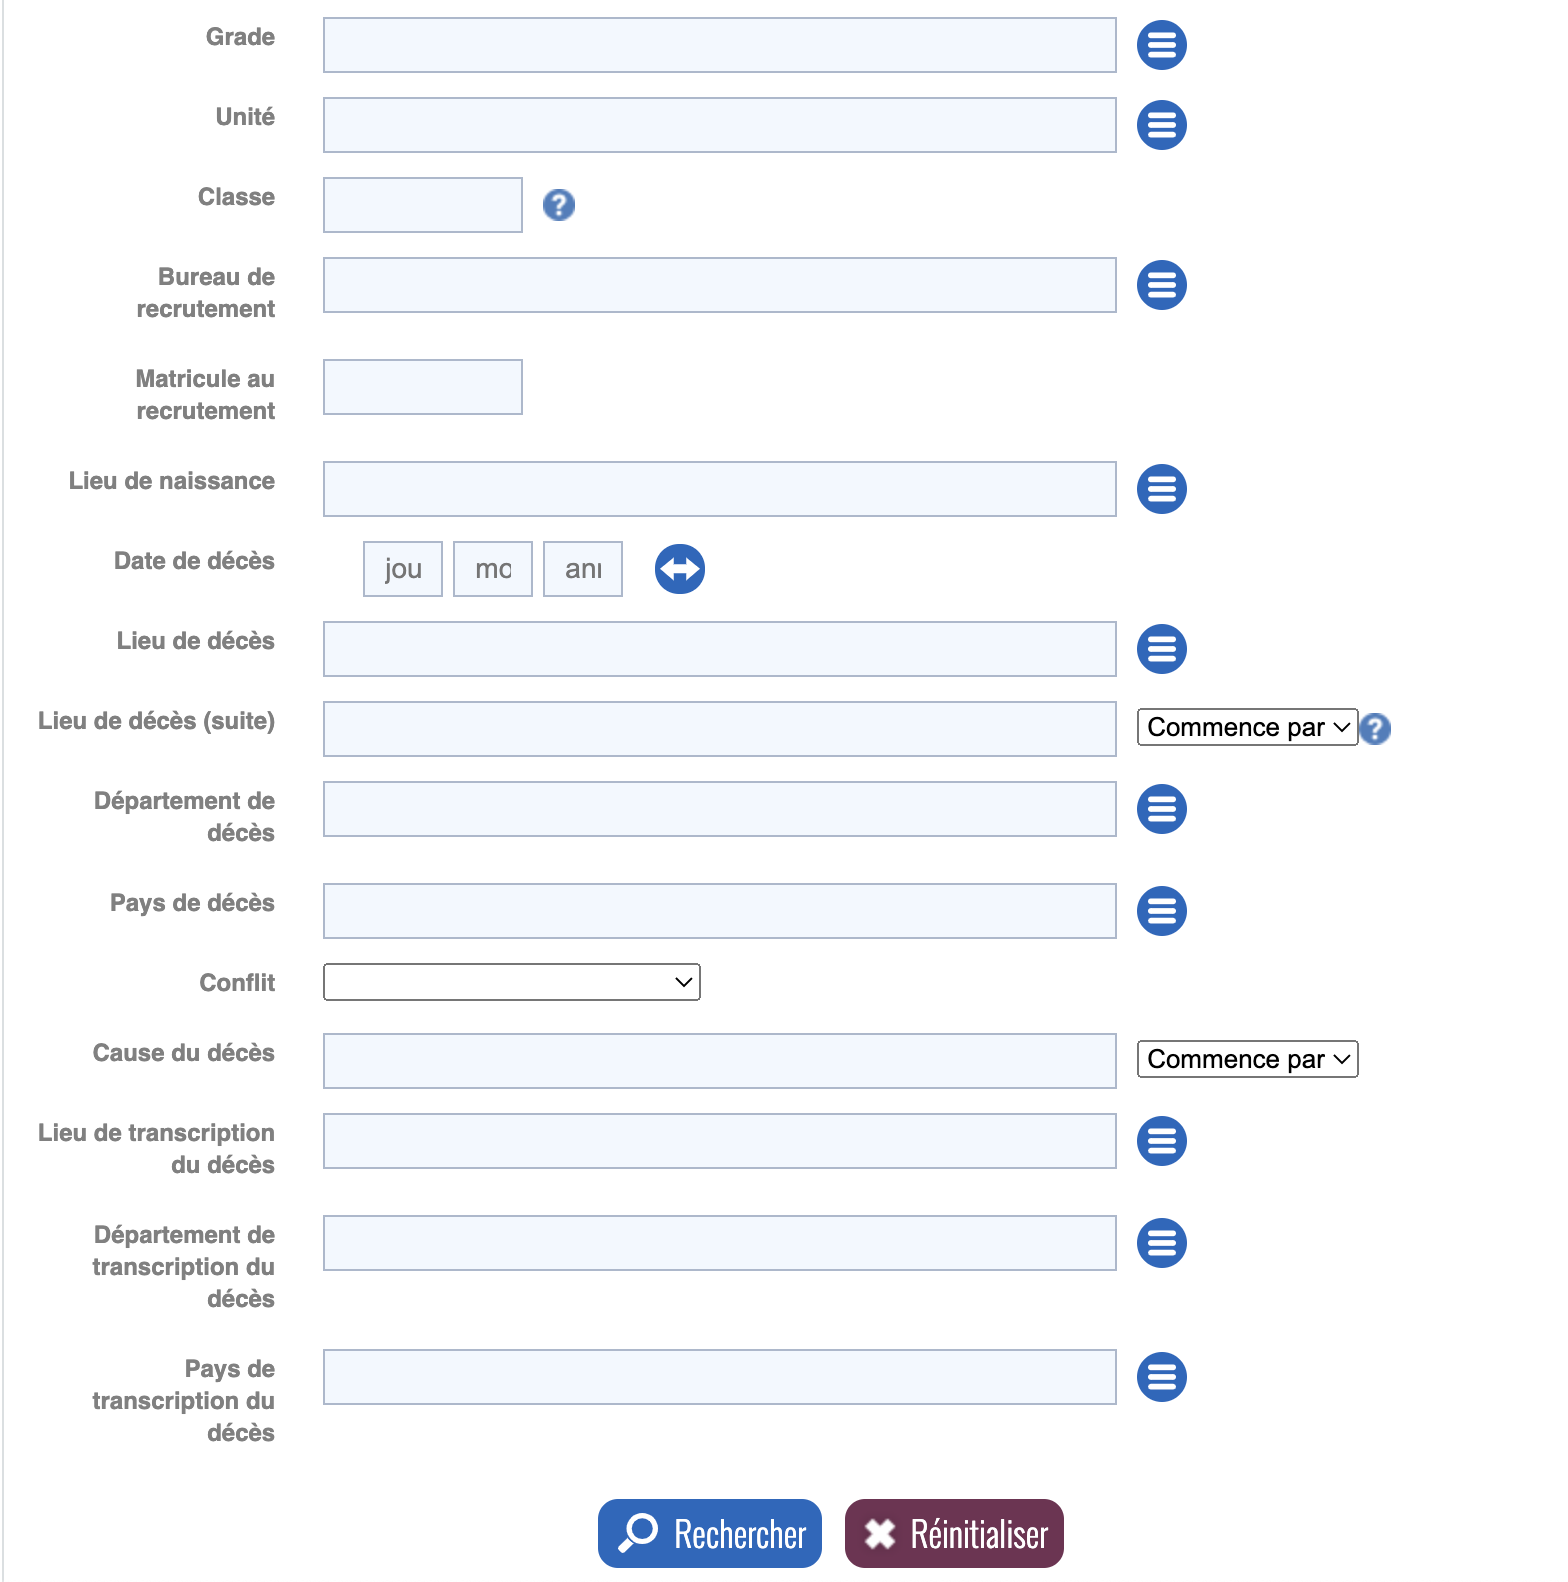
\includegraphics[scale=0.27]{ark2.png}
    \caption{Moteur de recherche avancé}
    \label{fig:Arkothèque 2}
\end{figure}

Le reste de mes resultats: 
\begin{figure}[h]
    \centering
    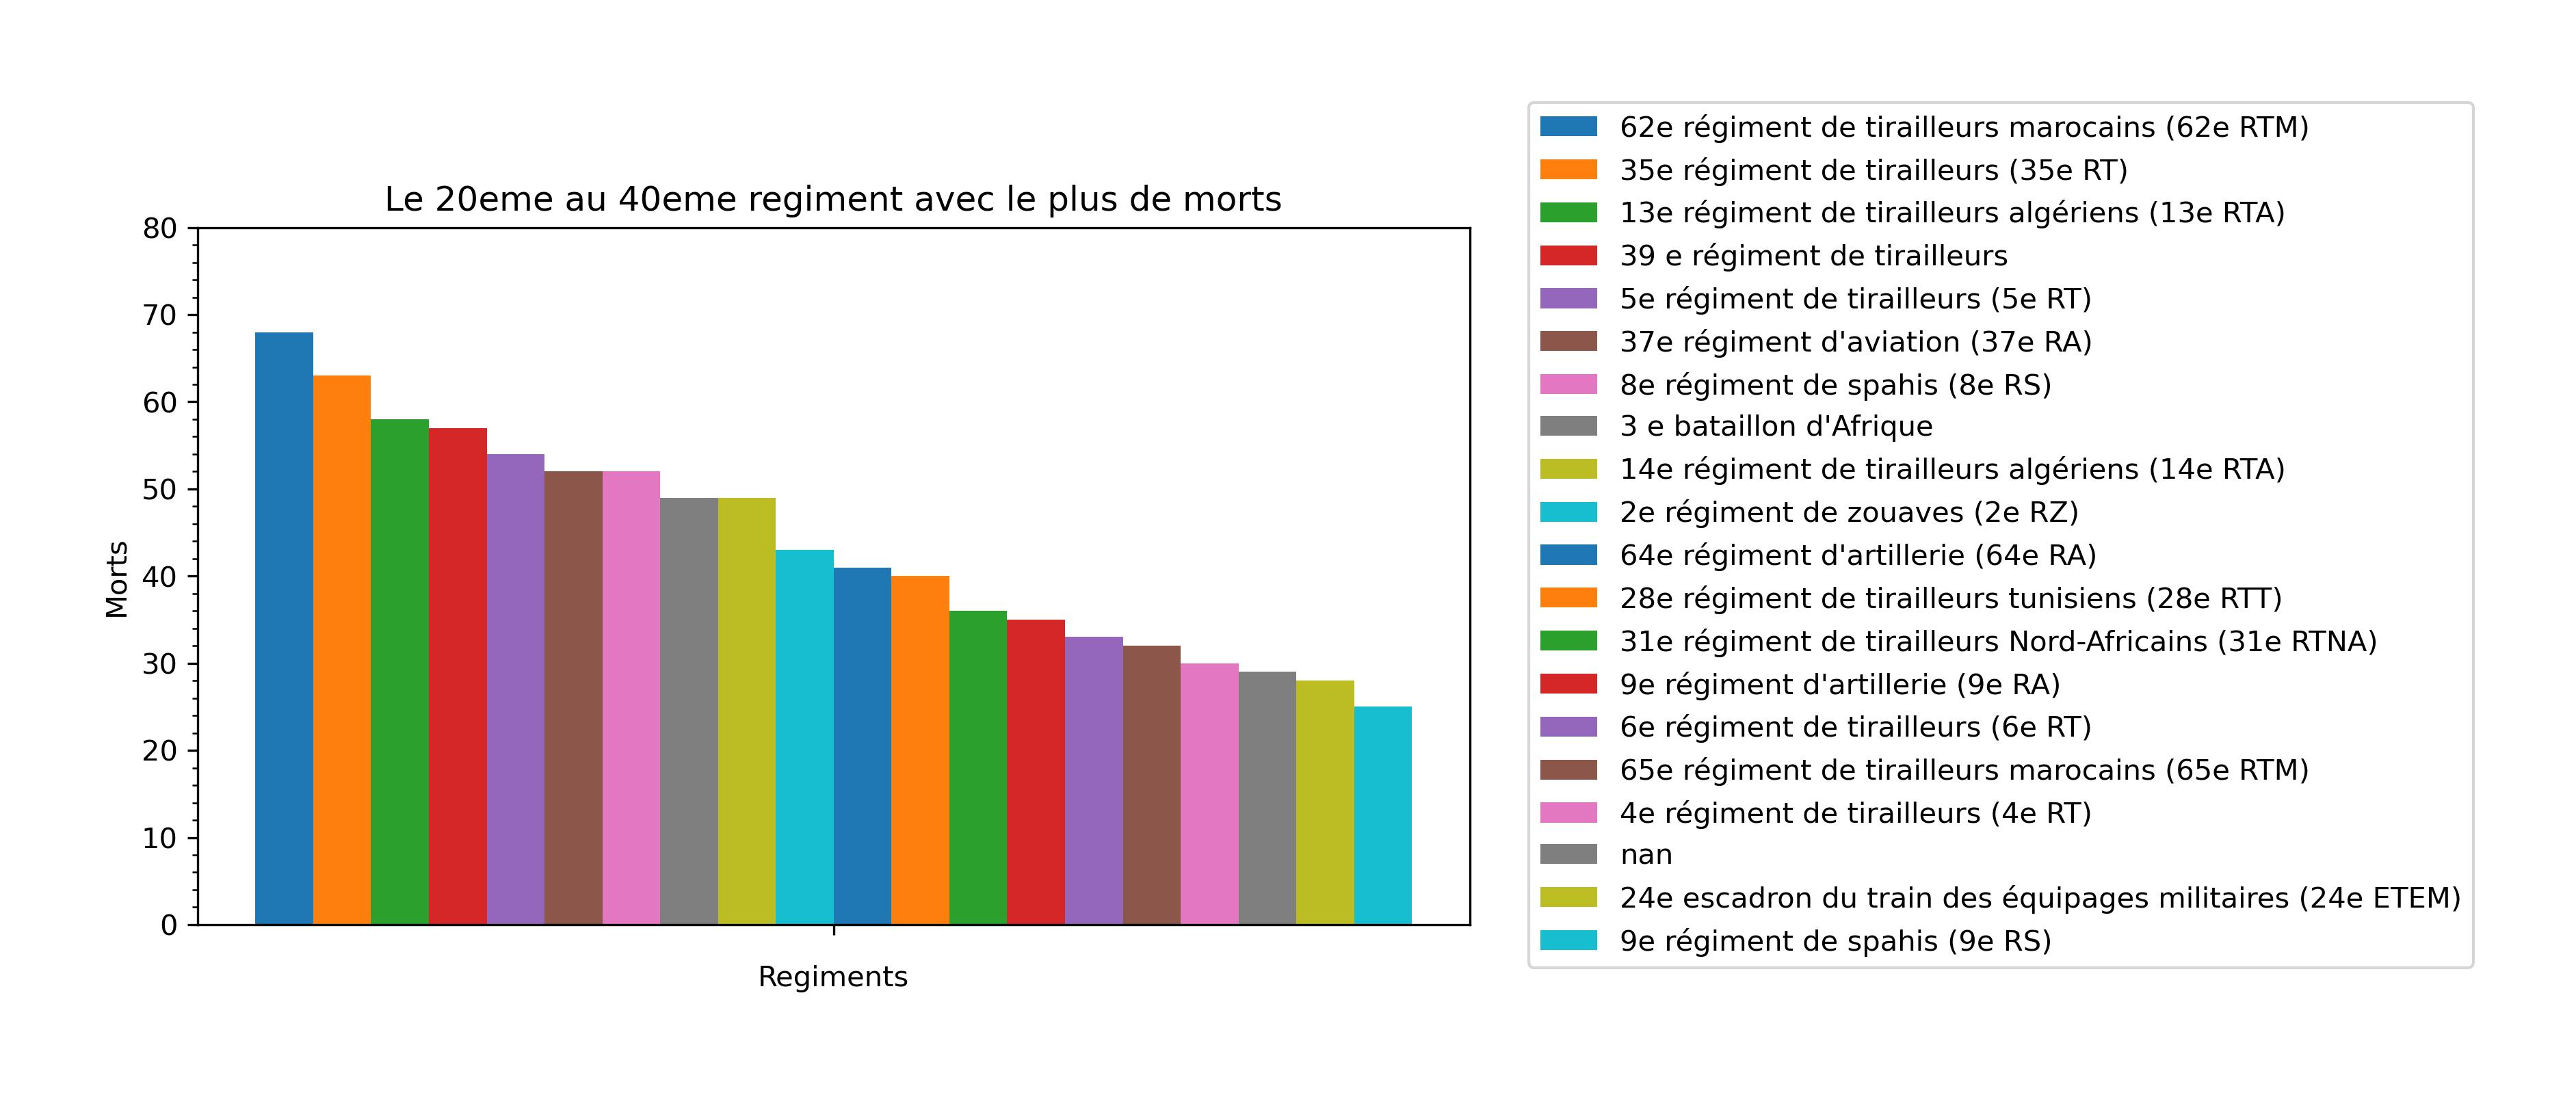
\includegraphics[scale=0.7]{Images/next20regiments.jpg}
    \caption{Les 20 à 40 régiments avec le plus pertes}
    \label{fig:Régiments 2}
\end{figure}
\begin{figure}[h]
    \centering
    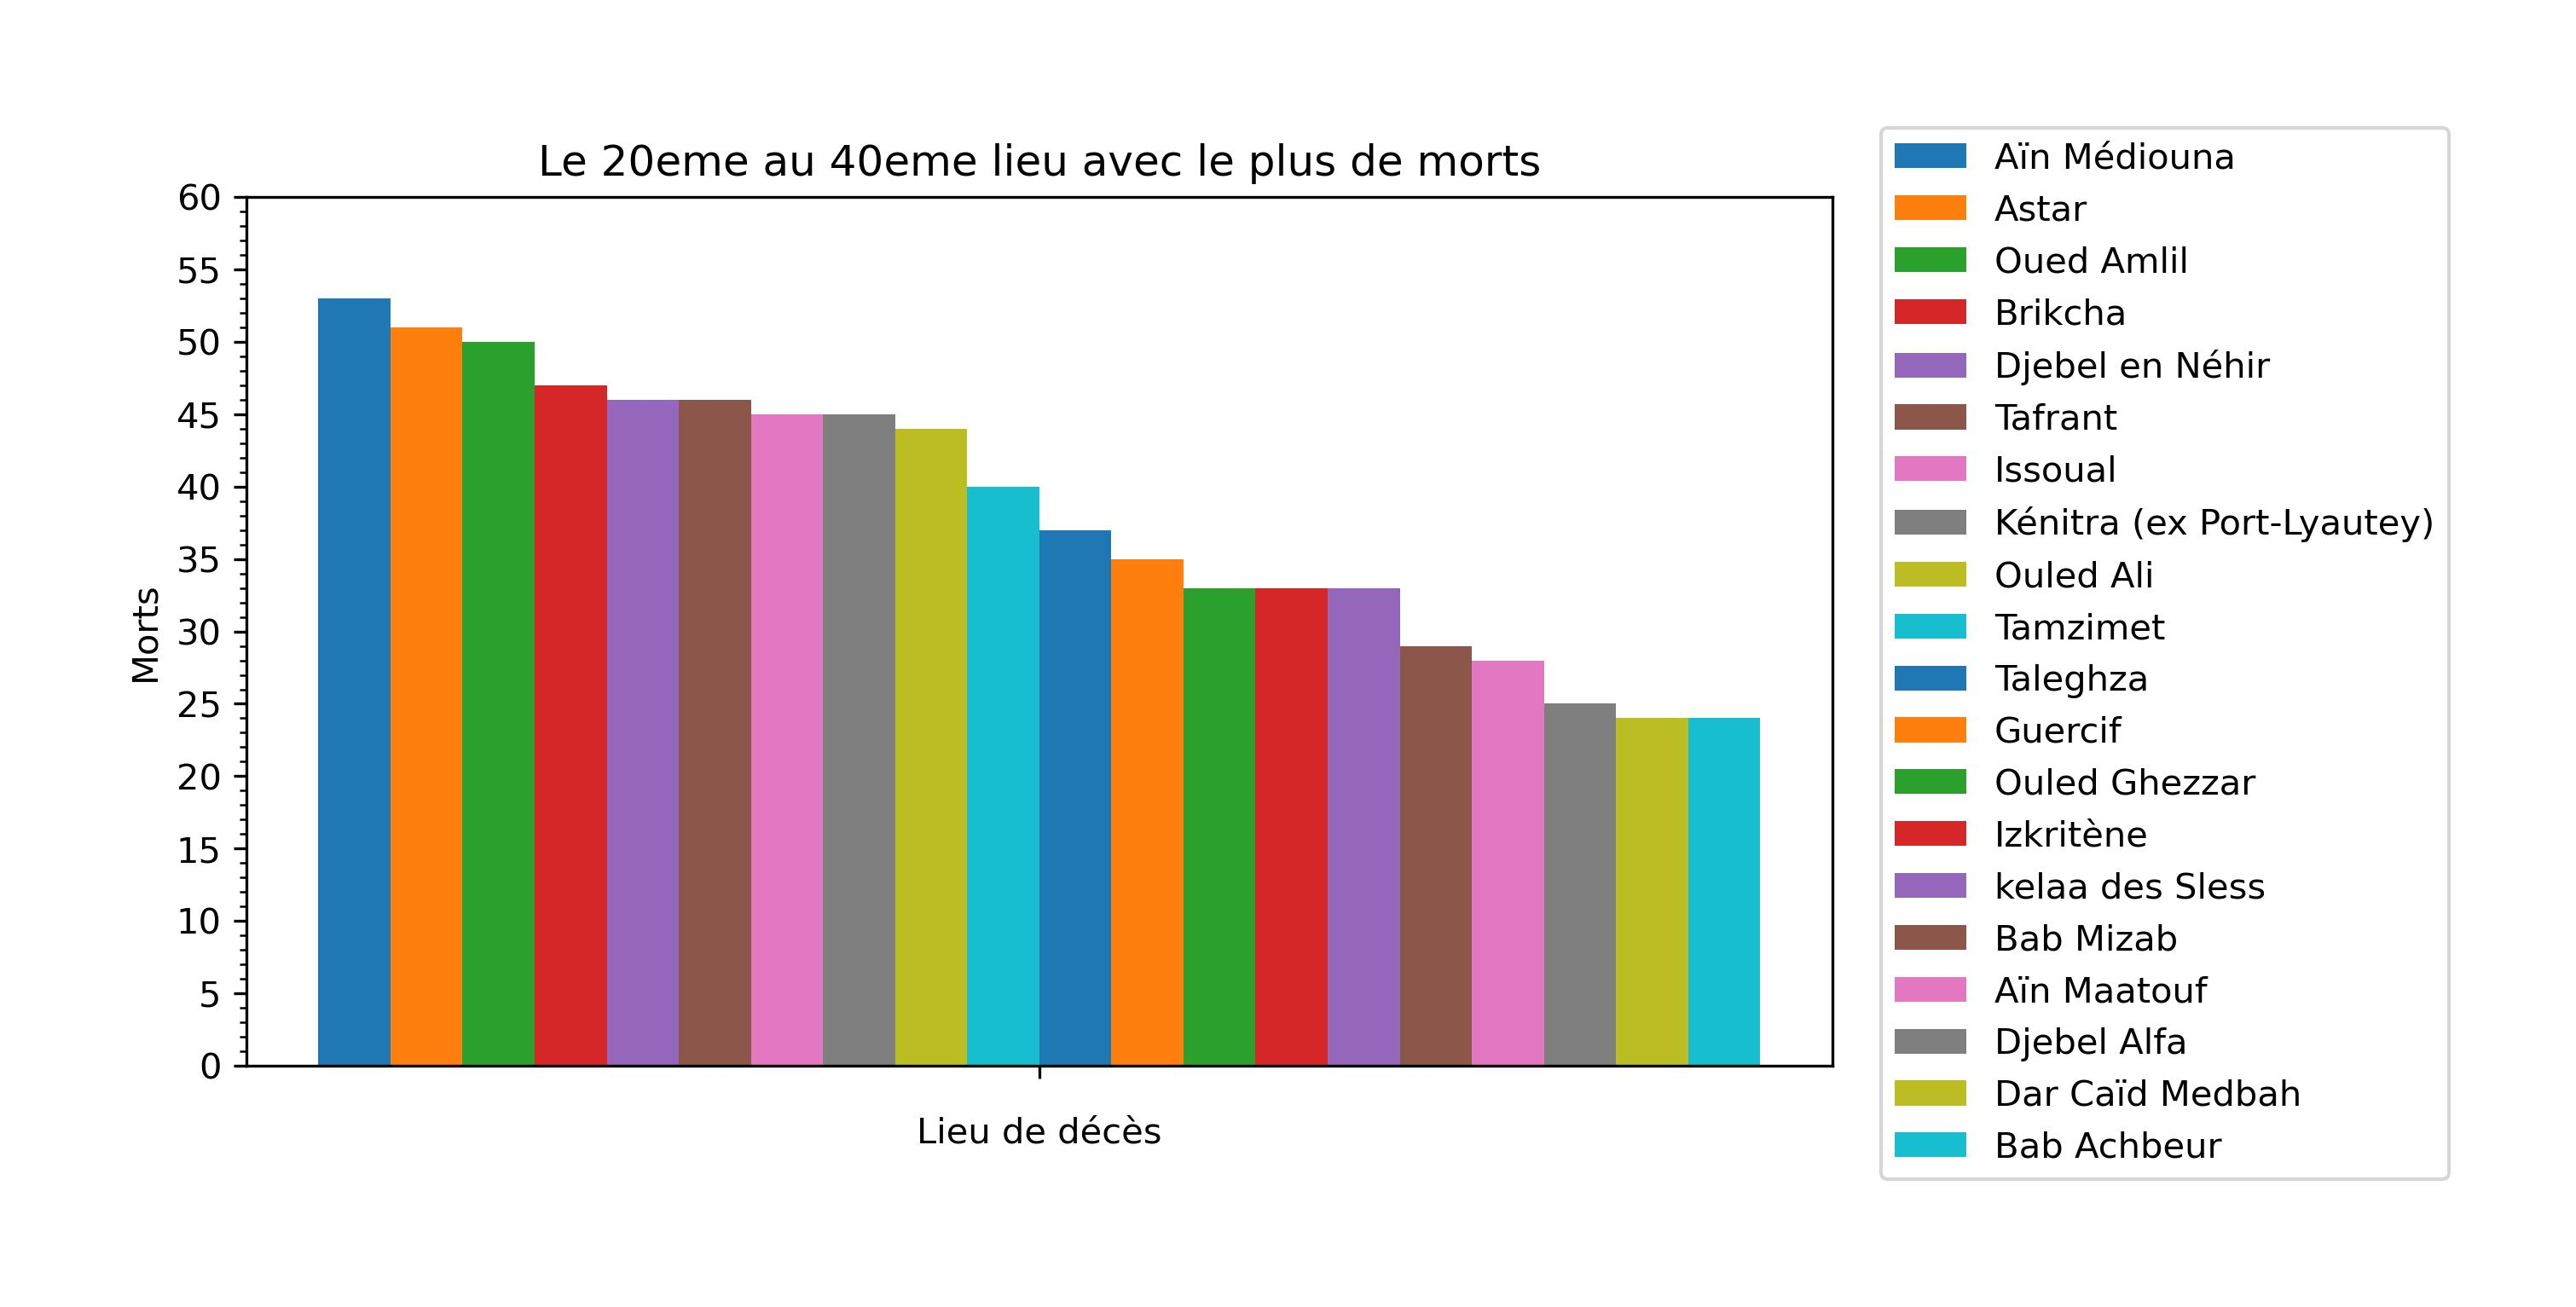
\includegraphics[scale=0.7]{Images/next20places.jpg}
    \caption{Les 20 à 40 lieux avec le plus pertes}
    \label{fig:Lieux 2}
\end{figure}
\begin{figure}[h]
    \centering
    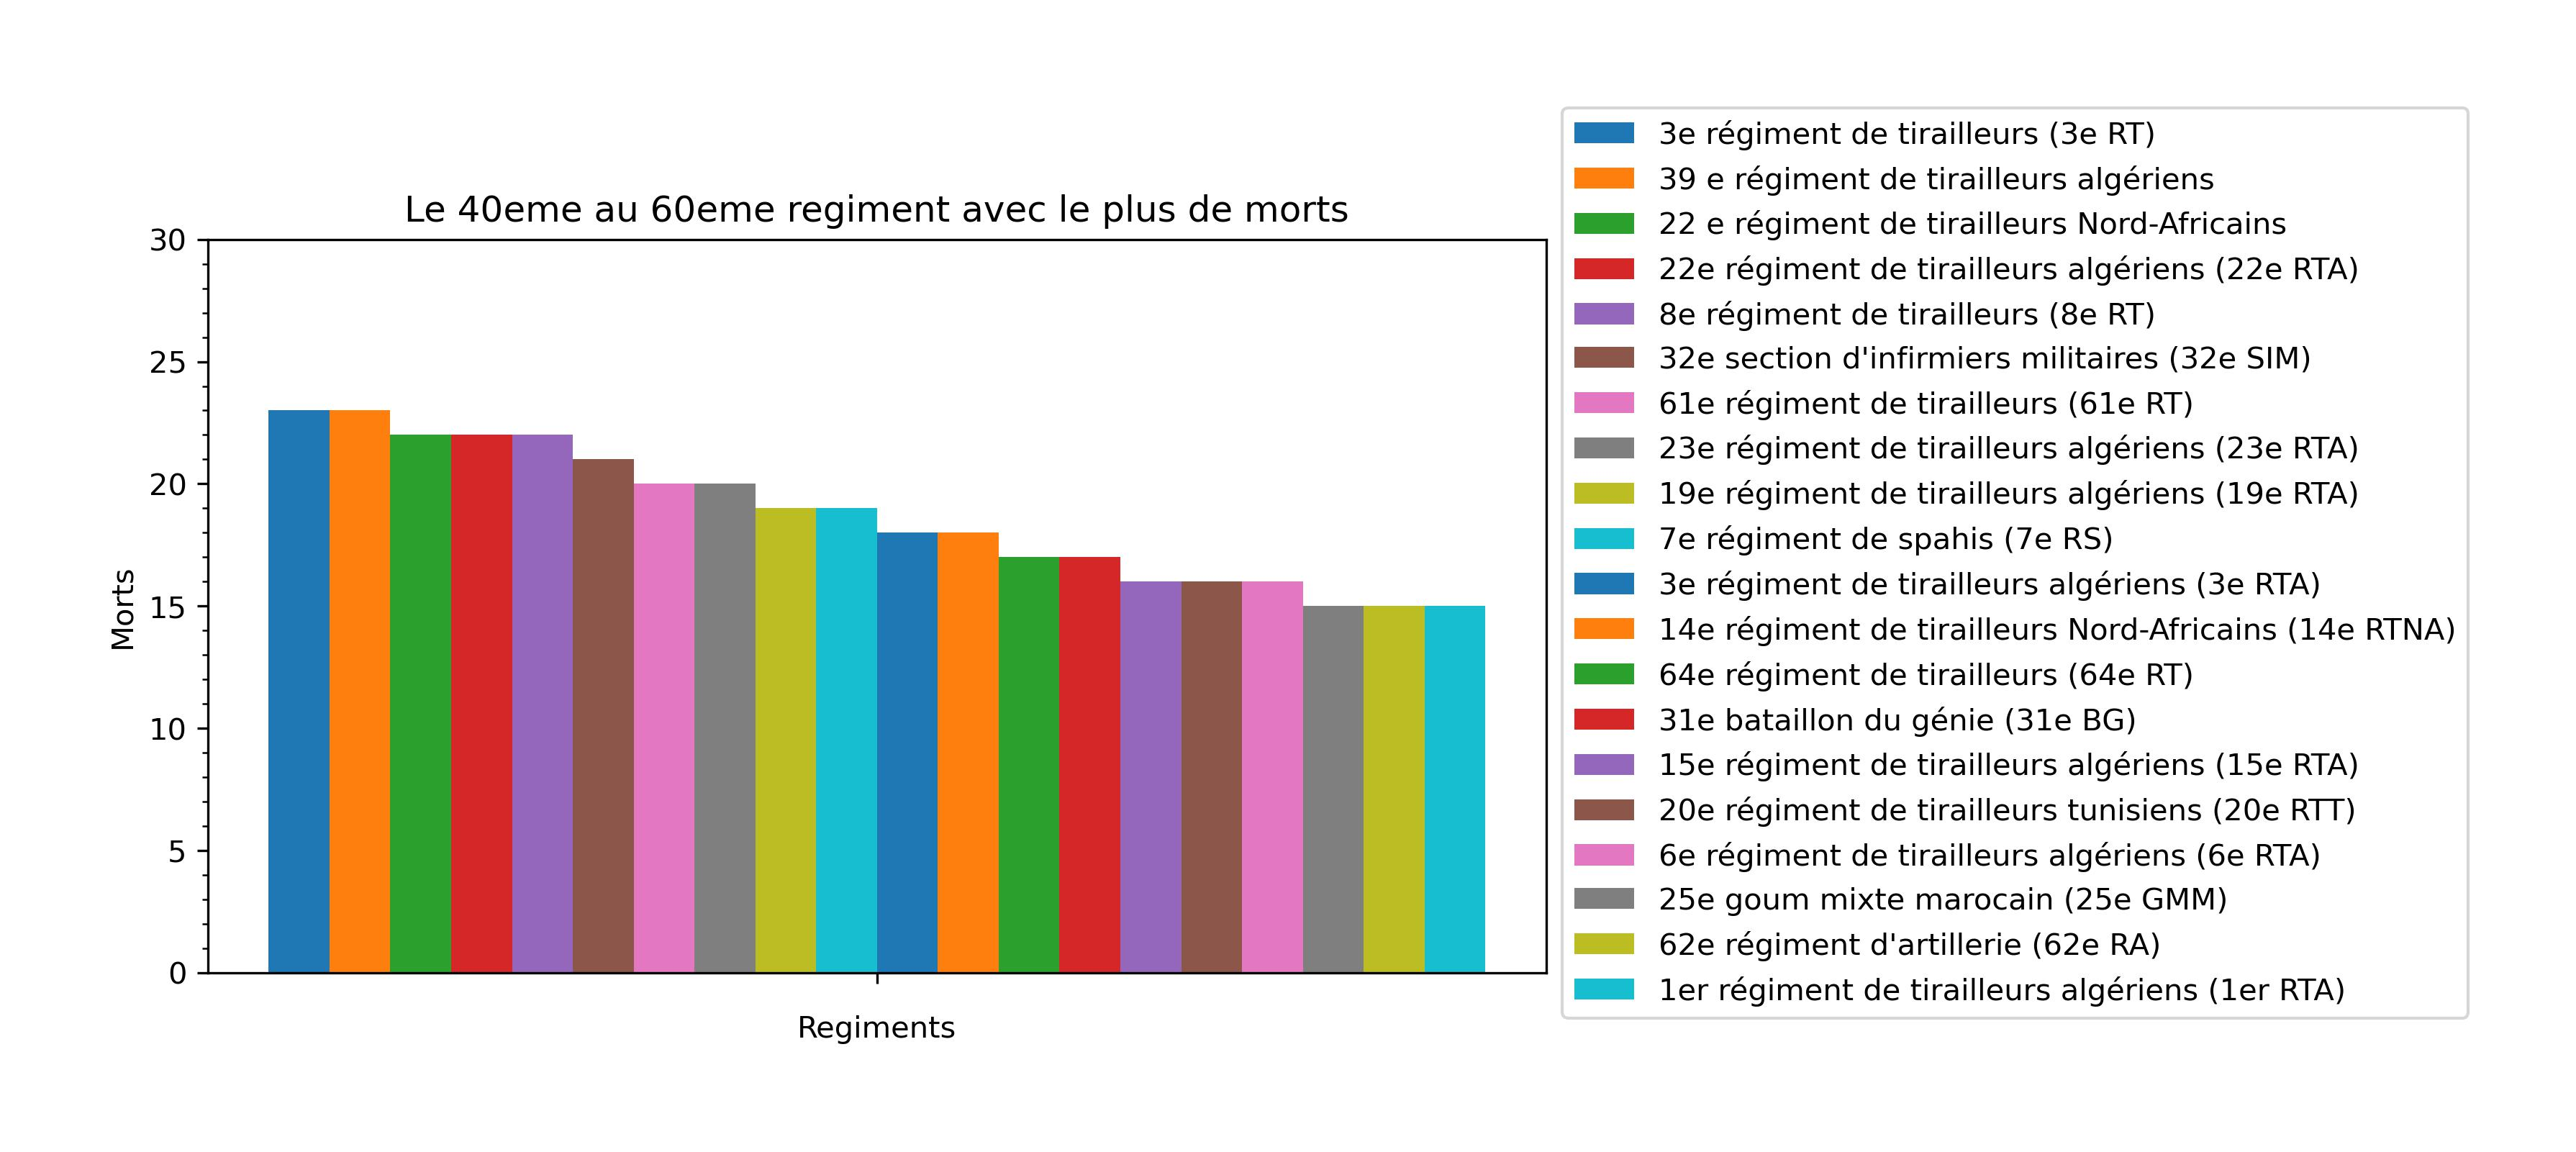
\includegraphics[scale=0.7]{Images/last20regiments.jpg}
    \caption{Les 40 à 60 régiments avec le plus pertes}
    \label{fig:Régiments 3}
\end{figure}
\begin{figure}[h]
    \centering
    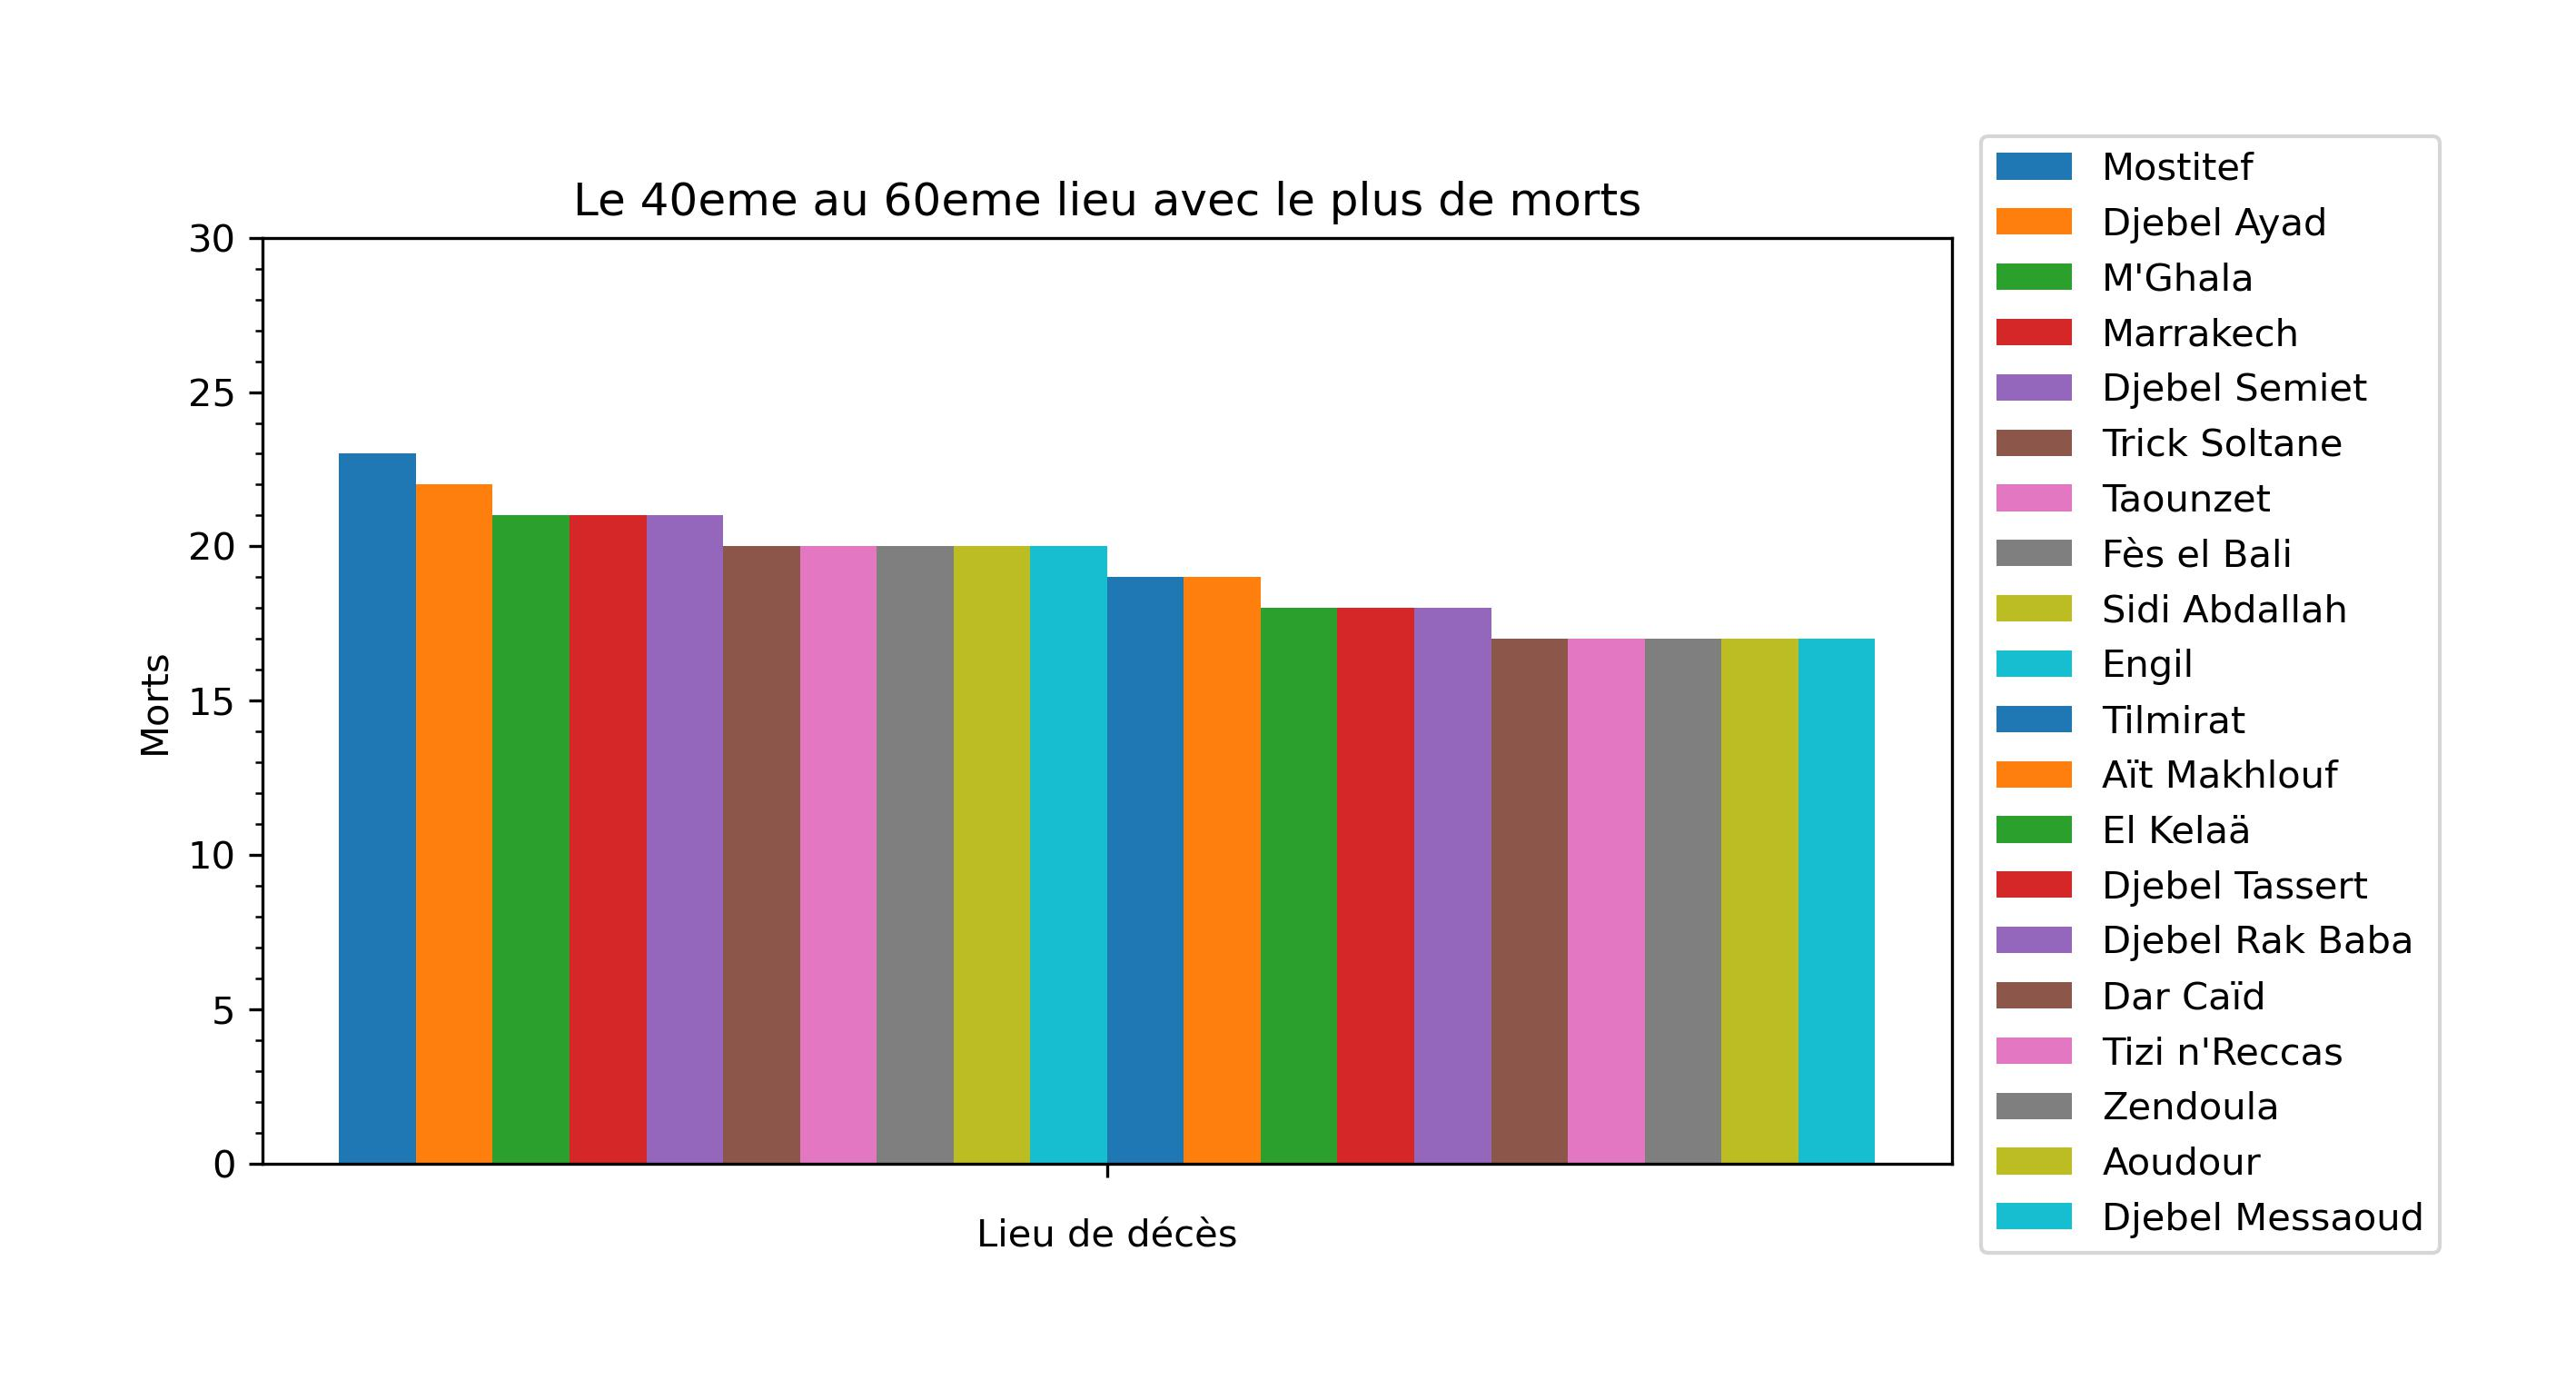
\includegraphics[scale=0.7]{Images/last20places.jpg}
    \caption{Les 40 à 60 lieux avec le plus pertes}
    \label{fig:Lieux 3}
\end{figure}
\begin{figure}[h]
    \centering
    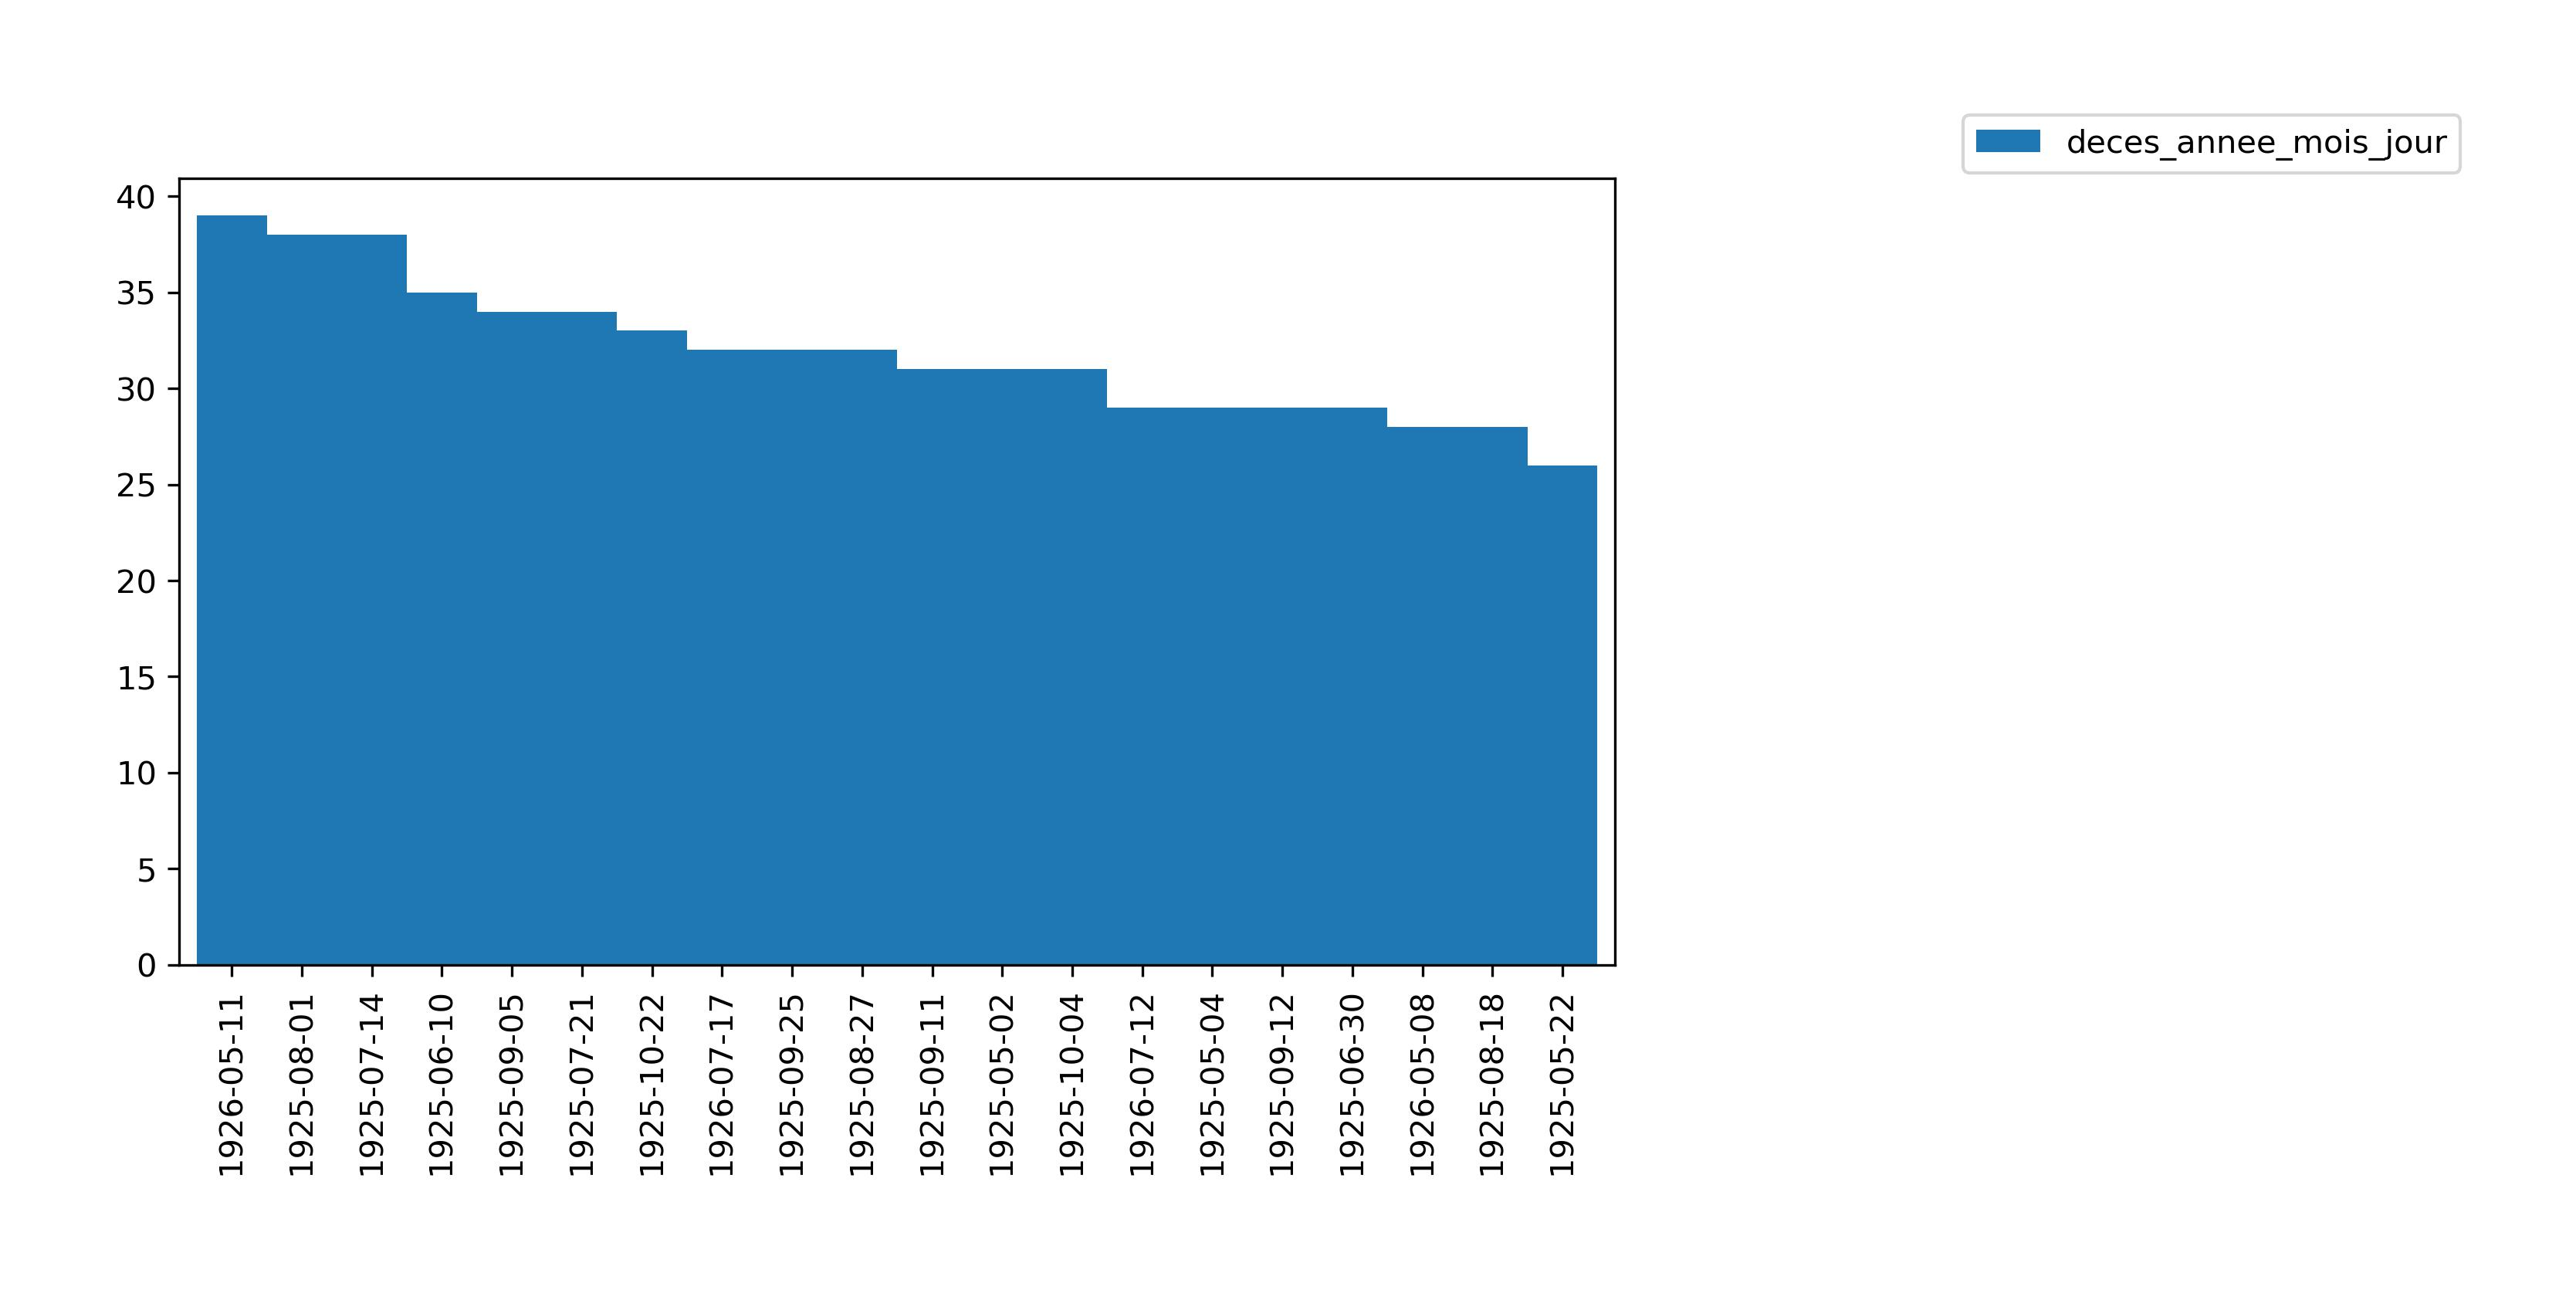
\includegraphics[scale=0.67]{Images/next20dates.jpg}
    \caption{Les 20 à 40 dates avec le plus pertes}
    \label{fig:Dates 2}
\end{figure}
\backmatter

\newpage
\nocite{*}
\printbibliography

% glossaire
%\include{back/glossaire}

% table des figures
\listoffigures

% table des matières
\tableofcontents

\end{document}